%% Short data paper template
%% Created by Simon Hengchen and Nilo Pedrazzini for the Journal of Open Humanities Data (https://openhumanitiesdata.metajnl.com)

\documentclass{article}
\usepackage[english]{babel}
\usepackage[utf8]{inputenc}
\usepackage{johd}
\usepackage{graphicx}
\usepackage{subcaption}
\usepackage[left=3.5cm, right=3.5cm]{geometry} % Margin

\title{Tracking Olympic Triumphs: A 120-Year Data Analysis}

\author{Carlos Lima, Henrique Beltrão, Jaime Carneiro,  Luís Novaes, Walléria Simões \\
        \small Fundação Getulio Vargas, Brazil \\\\
}
\date{}

\begin{document}
\maketitle
\begin{abstract} 
\noindent The Olympic Games are a global celebration of athletic excellence, uniting competitors from diverse backgrounds in elite competition. This paper offers an exploratory analysis of 120 years of Olympic data, focusing on demographic trends, economic factors, and athletic performance. Key aspects include the evolving age profiles of athletes, variations in physical characteristics across different sports, and the influence of national economic conditions on athletic success. Special attention is given to the performance of female athletes, examining trends in participation and outcomes over time. The findings provide a comprehensive view of the evolving dynamics that shape Olympic competition, with insights into the factors influencing success at the highest levels of sport.\end{abstract}

\noindent\keywords{Olympic Games; Demographic trends; Inclusion in sports; Economic factors}\\

\section{Introduction}

The Olympic Games, held every four years, bring together athletes from countries around the world to compete at the highest level of international sport. The Olympics are a global event, symbolizing athletic excellence and unity among nations.

The origins of the Olympics trace back to ancient Greece, where the Games, known as the Ancient Olympic Games, were held on the sacred grounds of Olympia. These early Games took place from approximately 776 B.C. to 393 A.D., serving as a key cultural and religious event for the Greeks. The modern Olympic Games, revived in 1896, were envisioned as a unique opportunity for international reconciliation and sporting achievement. Over the 20th century, the Olympics grew exponentially in size, influence, and significance, establishing themselves as "the greatest spectacle on Earth."

Comparing the first modern Olympic Games in Athens in 1896 with the centennial edition in Atlanta in 1996 reveals a remarkable transformation. Over that century, the number of sports, participating countries, athletes, and spectators surged dramatically. There was also notable progress in training techniques, technological advancements in sports science, and improvements in athletic performance. Additionally, the growing inclusion of women and the increasing diversity of races and ethnicities reflected broader social changes \cite{Lancelotti}.

Women’s participation in the Olympic Games was officially recognized by the International Olympic Committee (IOC) in 1919, although initially limited to swimming and tennis. Track and field events, symbolizing the core of Olympic competition, remained exclusively male. In response to this exclusion, Alice de Milliat, an athlete and women's rights activist, founded the French Sports Federation (FEF) in 1917 and later established the International Women's Sports Federation (FEFI). These efforts were motivated by resistance from the International Amateur Athletic Federation (IAAF) and opposition from key figures like Pierre de Coubertin, who sought to limit women’s involvement in athletics \cite{devide2005}.

Sporting events around the world not only mobilize vast sums of money but also capture the passions of millions of sports enthusiasts. Among these events, the Summer Olympic Games stand as the largest and most traditional, featuring numerous sports and bringing together nations in a unified celebration of competition. Hosting such an event requires robust infrastructure and significant economic resources, underscoring the substantial impact these games have—not only in terms of the preparation and training required by participating athletes but also in the enormous investments made by the host country, often amounting to billions, to ensure the event's success and attract a global audience.

The 2016 Rio de Janeiro Olympics serve as a prime example. A study by the Getulio Vargas Foundation (FGV), titled "Legacy of the Rio 2016 Olympic Games: Economic Impacts" \cite{FgvConhecimento}, published in July 2024, highlights the economic activities catalyzed by the event. According to the study, the Games contributed R\$ 99 billion to the Gross Production Value (GPV) of the region, of which R\$ 51.2 billion was added to the GDP. Additionally, tax revenues increased by R\$ 5.3 billion, and household income experienced a boost of R\$ 36.2 billion. These figures illustrate the enduring economic legacy the Olympics can leave on a host city.

Alongside the Olympic Games, the Paralympic Games represent another monumental international event, featuring elite athletes from delegations worldwide. Taking place every four years, the Paralympics involve athletes with physical disabilities, reflecting the inclusive nature of global sports. The origins of the Paralympics date back to the aftermath of World War II, as Dr. Ludwig Guttmann sought to improve the quality of life for injured soldiers by introducing them to adaptive sports \cite{paralimpiadas}. This initiative laid the foundation for what would become one of the world's most significant sporting movements . This paper aims to examine the role of the Paralympics in contemporary society, particularly with regard to the visibility and impact of these games.

In this study, we conducted an in-depth analysis of the aforementioned factors and their potential correlations with athlete performance in both the Olympic and Paralympic competitions. The dataset employed for this analysis was sourced from various reliable databases and contains detailed information about athletes, including age, gender, sport, and competitive outcomes. The dataset enabled the production of descriptive statistics that provided a richer understanding of the athletes' profiles. Moreover, external factors such as the economic conditions of the countries and levels of urbanization were explored, aiming to uncover how these elements might influence sporting success. This holistic approach allows for a comprehensive analysis, contributing to a broader understanding of the dynamics that underpin Olympic and Paralympic competitions.

\section{Method}

\paragraph{Steps} Initially, we selected a dataset containing information about athletes who participated in the Olympic Games between 1896 and 2016 \cite{120_anos_olimpiadas}. This dataset included details such as the athletes' names, countries represented, sports modalities, and physical characteristics like age, height, and weight. To provide a more comprehensive analysis, we also incorporated datasets from Paralympic competitions \cite{paralimpiadas_verao_inverno} and external data on the urbanization levels \cite{urbanizacao_paises} and GDP of the athletes' home countries \cite{pib_paises}. The inclusion of these additional datasets enriched the analysis by allowing us to explore correlations between socioeconomic factors, national development levels, and the athletes’ performances in both the Olympic and Paralympic events.

\paragraph{Data Treatment} One of the first challenges we faced during the data cleaning process was the presence of missing values for certain physical characteristics (height, weight, and age) for some athletes. Since these are numerical variables, we used a Linear Regression Algorithm with the scikit-learn Python library to predict the missing values based on the available data from other athletes with similar profiles. This method enabled us to fill in the gaps consistently, ensuring the dataset’s integrity for further analysis.

To facilitate comparisons, we standardized the types of medals (Gold, Silver, Bronze, and Non-Medalists) by assigning ordinal qualitative values: Gold received a weight of 3, Silver a weight of 2, Bronze a weight of 1, and Non-Medalists a weight of 0. This approach enabled a clearer comparison of performance across genders, allowing for a more accurate assessment of competitive success between different kinds of athletes.

During this analysis, we faced the challenge of standardizing the dataframes, particularly between the Olympic athletes dataset and the dataset containing urbanization data over time. To maintain the integrity of the analysis without losing relevant data, it was essential to normalize the country names to accurately align the information between the two datasets, especially given that urbanization data were only available from 1950 to 2020 (with projections for up until 2050).

\section{Analysis}

\subsection{Age Analysis}
\paragraph{First Look}
We selected the athletes' Age as one of the key variables for analysis. \\
Descriptive Statistics of the 'Age' Column in the Dataset:

\bigskip
\scalebox{0.83}{
\begin{center}
\begin{tabular}{|c|c|c|c|c|c|c|c|c|c|}
    \hline
     Count & Mean & Std. Deviation & Min &  Lower Lim & Quartile 1 & Med & Quartile 3 & Upper Lim & Max \\ \hline
    271016 &  25.61 &  6.37 & 10 & 13 & 22 & 25 & 28 & 37 & 97 \\ \hline
\end{tabular}
\end{center}
}
\bigskip

While examining the data, several questions arose:
\begin{itemize}
    \item Who are the athletes corresponding to the minimum and maximum recorded ages?
    \item Which sports have the highest number of outliers in terms of age?
    \item What is the age profile of Brazilian athletes?
    \item Is there a correlation between an athlete's age and their chances of winning a medal?
\end{itemize}

The analysis of the descriptive statistics for the athletes' ages revealed that the youngest recorded athlete was Dimitrios Loundras \cite{olympedia}, a Greek gymnast who competed in the 1896 Summer Olympics in Athens, winning a bronze medal \cite{OlympicsDimitri}. At 10 years old, he remains the youngest Olympic medalist in history, excluding competitors of unknown ages who acted as coxswains during the 1900 Olympics.

Interestingly, while Dimitrios is classified as an outlier when considering the age of all athletes across the Games, he falls within the normal age range expected for gymnasts. This difference in classification highlights the importance of evaluating data within specific contexts, as what might be an outlier in a general analysis could be typical in a narrower group.

Among the three sports with the most outliers, gymnastics stands out, followed by athletics and cycling.

\begin{figure}[H]
\centering
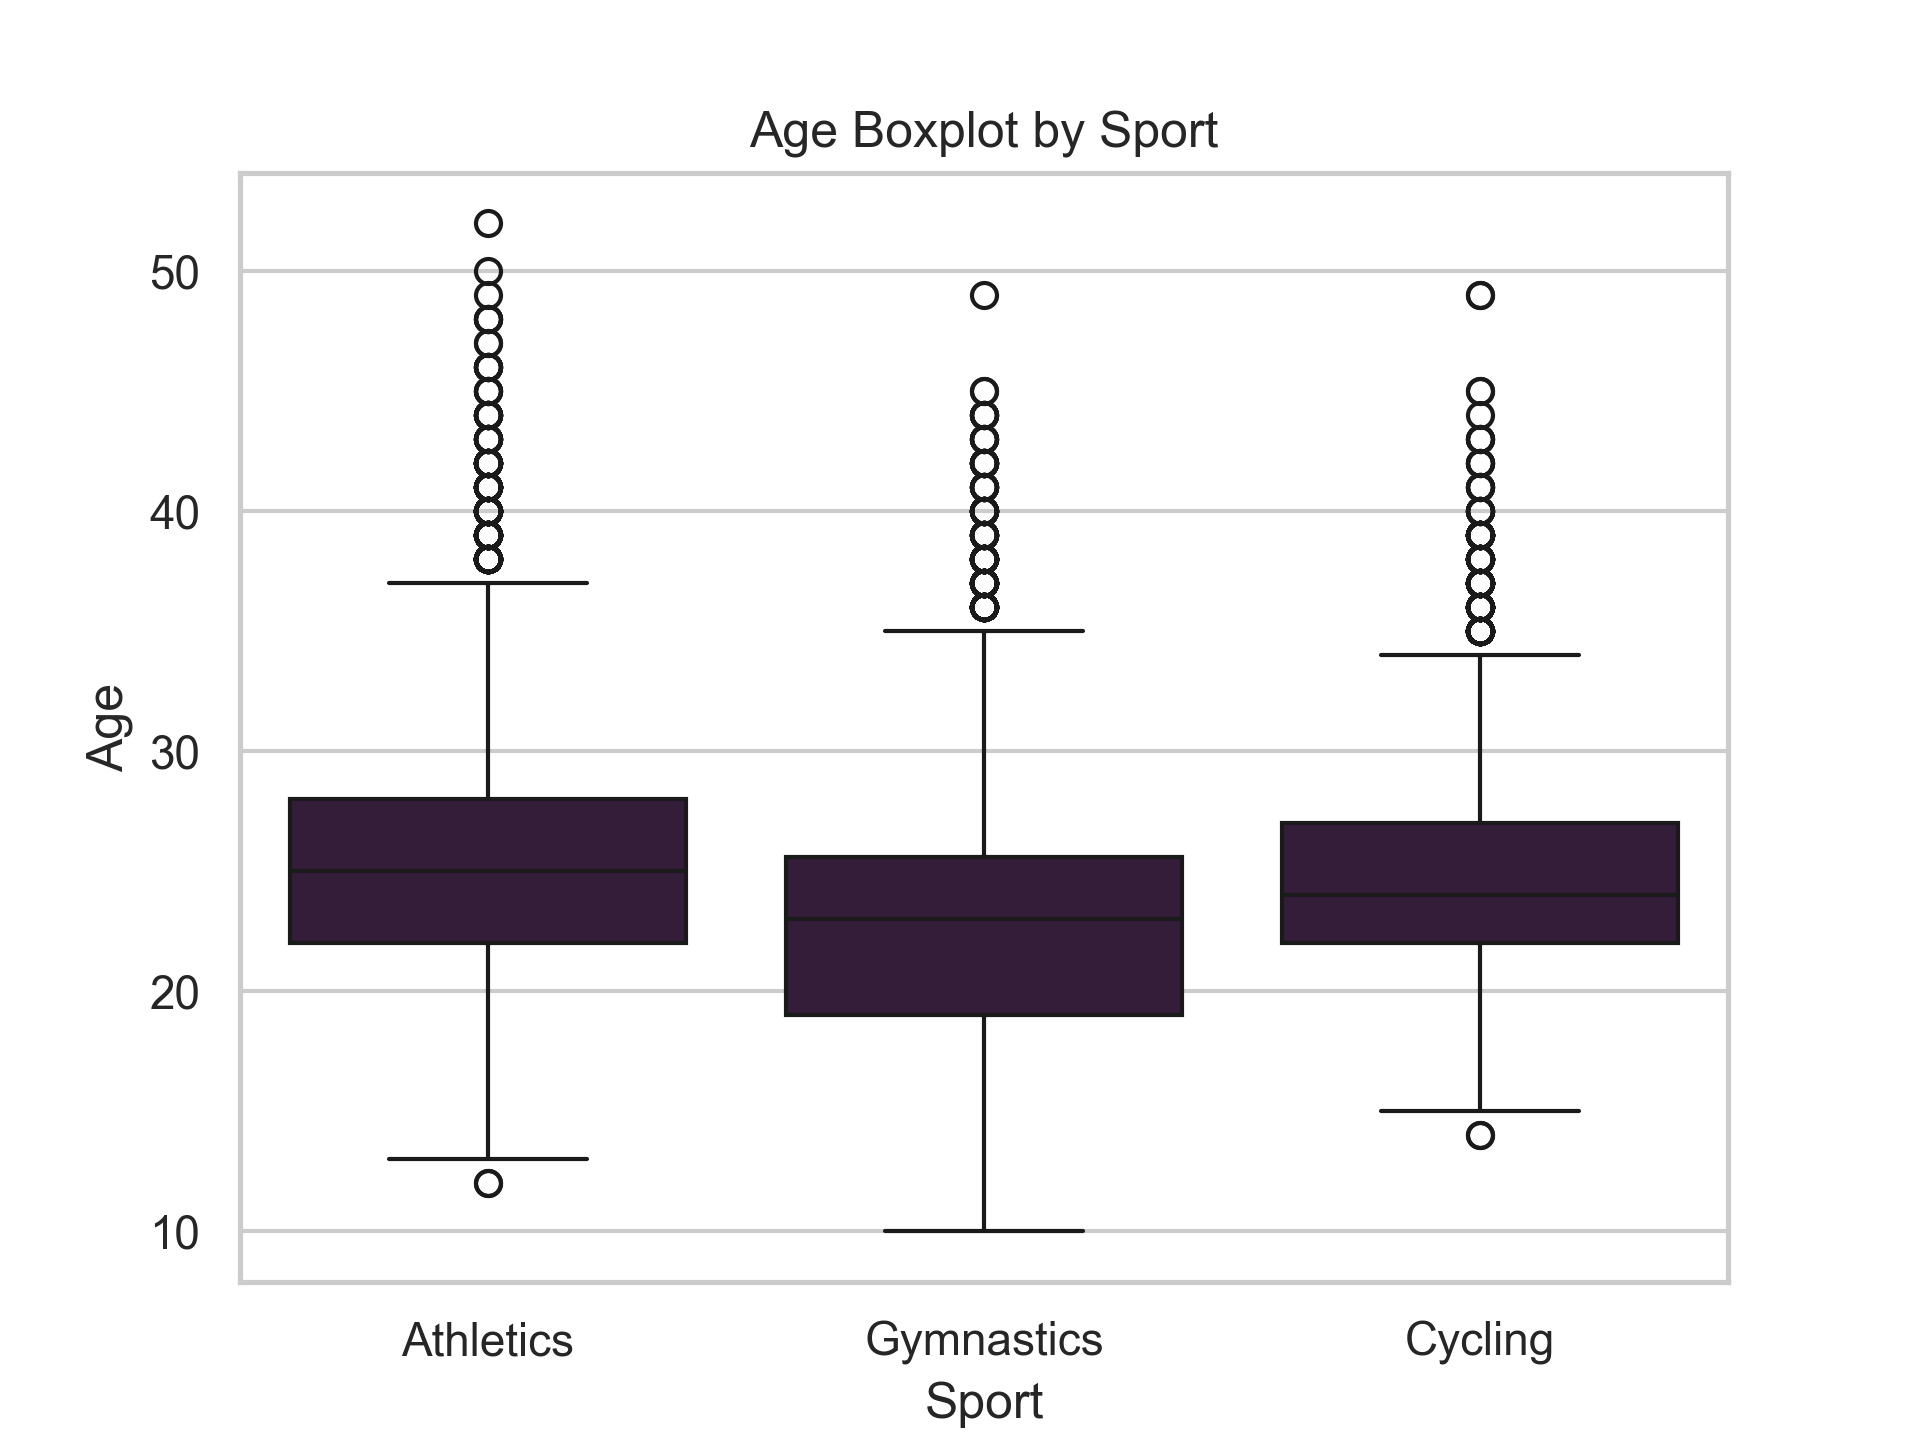
\includegraphics[width=0.7\textwidth]{images/age_analysis/bloxplot_top_3_highest_age_aplitude.png}
\caption{\label{fig3}Boxplot of Sports with the Highest Amount of Outliers}
\end{figure}

In sharp contrast, the oldest recorded participant was John Quincy Adams Ward, who at 97 years old submitted his sculpture posthumously for the 1928 Art Competitions in Amsterdam, making him the oldest competitor in Olympic history. These extremes provide important insight into the age range of the study's participants and the potential implications for their performance.

\paragraph{Brazilian Athletes and Age}
For Brazilian athletes, we analyzed those who received awards (medals) and those who did not. By calculating the coefficient of determination (R²) for these two categories in relation to age, we obtained a value of 0.000157. This result suggests a weak correlation between the athletes' age and their chances of winning a medal, indicating that age is not a significant factor in determining success among the Brazilian competitors analyzed.

\begin{figure}[H]
\centering
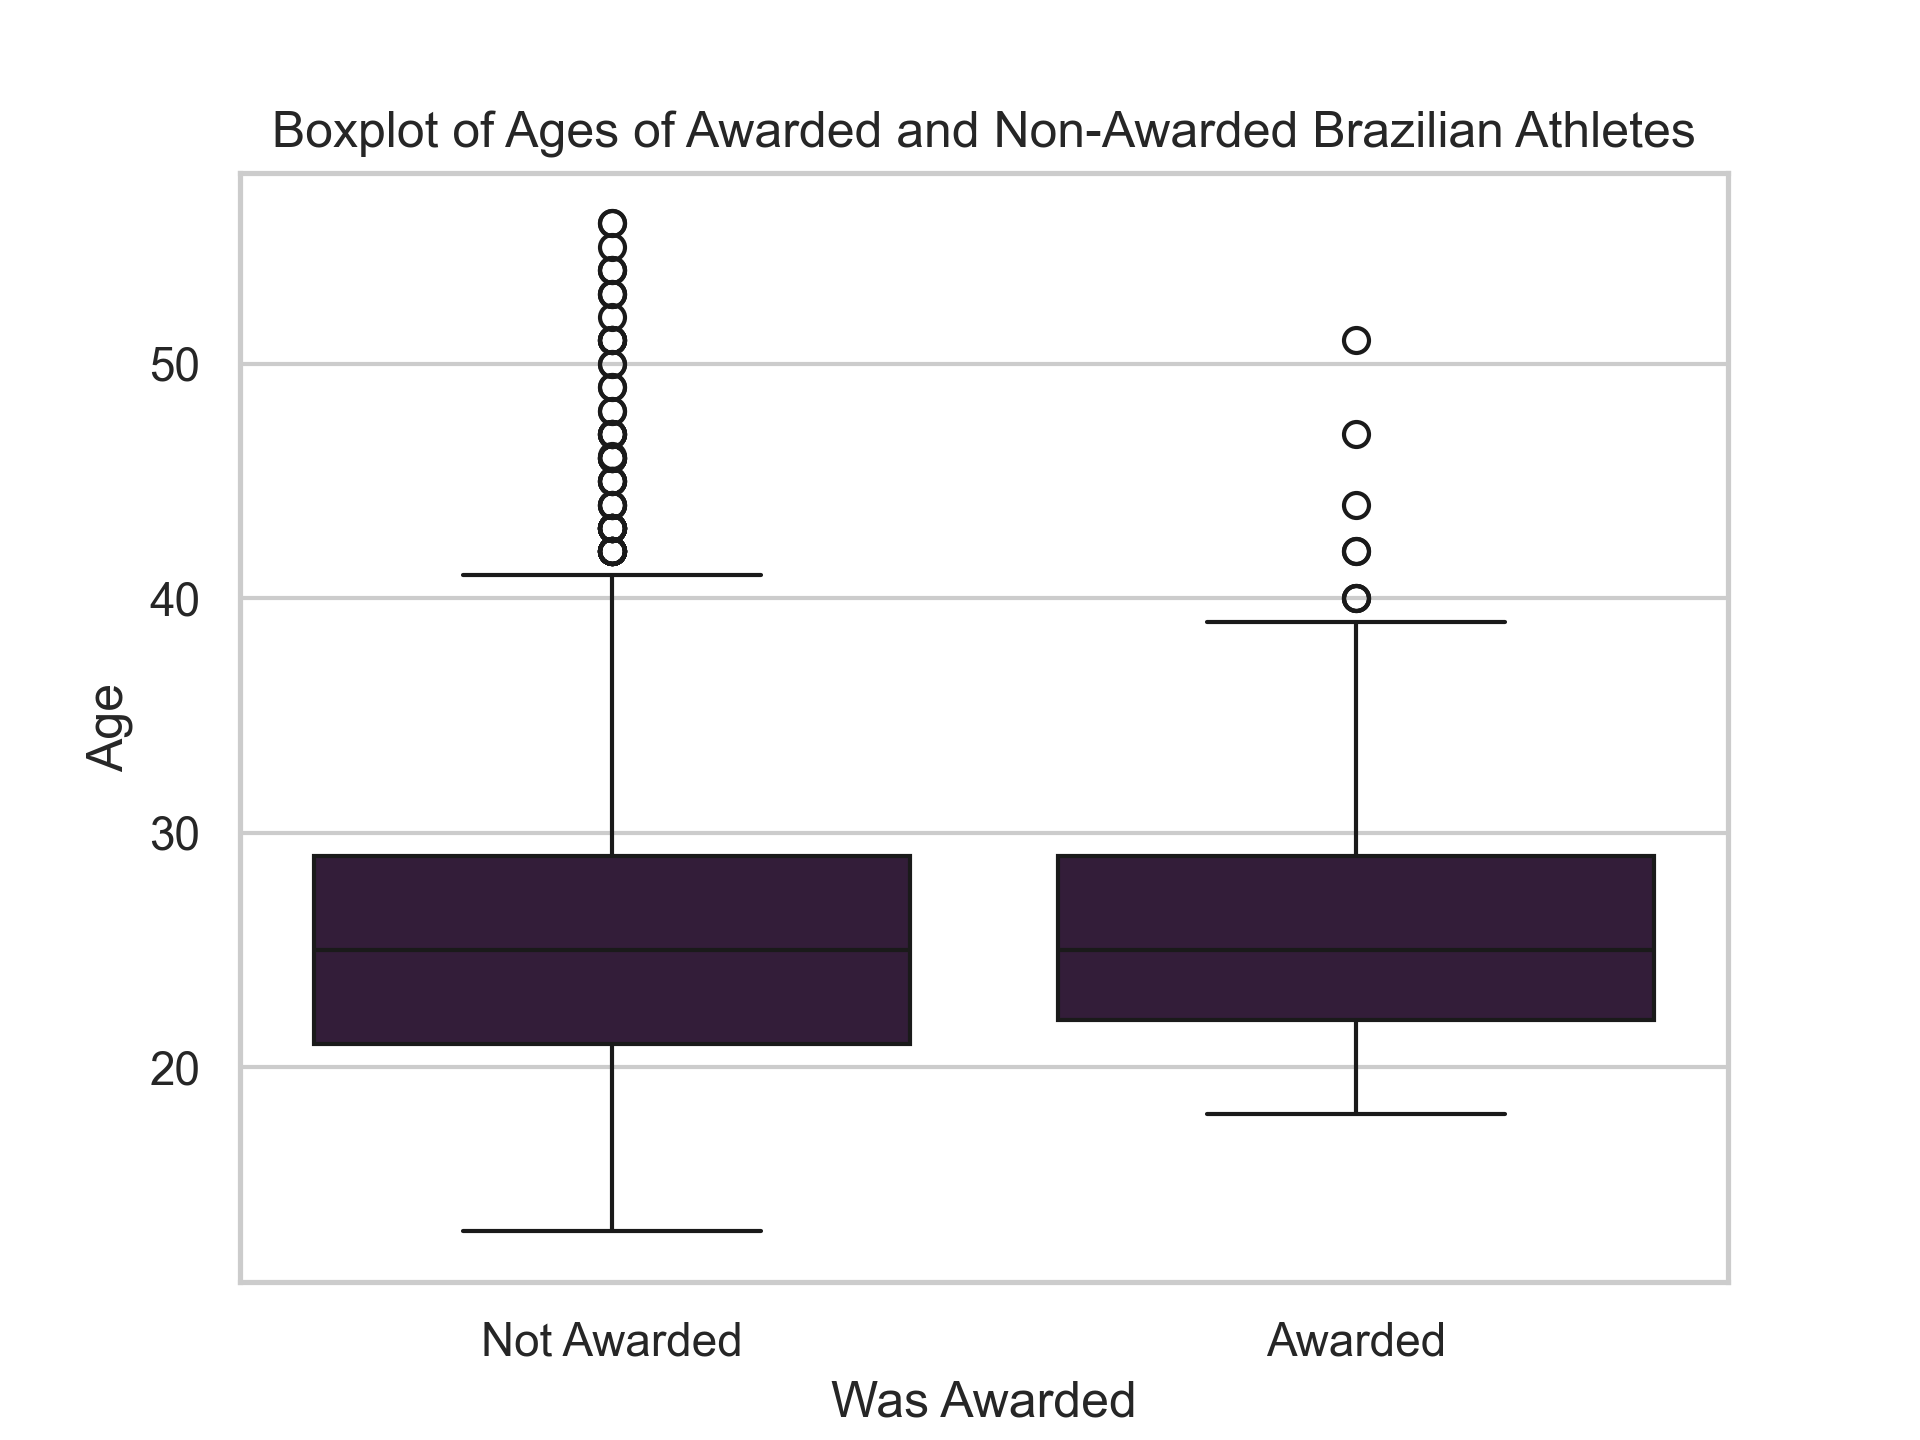
\includegraphics[width=0.5\textwidth]{images/age_analysis/boxplot_age_awarded_and_non_awarded_brazil.png}
\caption{\label{fig3}Boxplot with Medal Status of Brazilian Athlete's Ages}
\end{figure}

Each athlete was also characterized according to their sport. For this aspect of the analysis, the calculated R² coefficient was 0.336, indicating a stronger relationship between the age of Brazilian athletes and the sport they competed in, compared to the relationship between age and winning medals.

\begin{figure}[H]
\centering
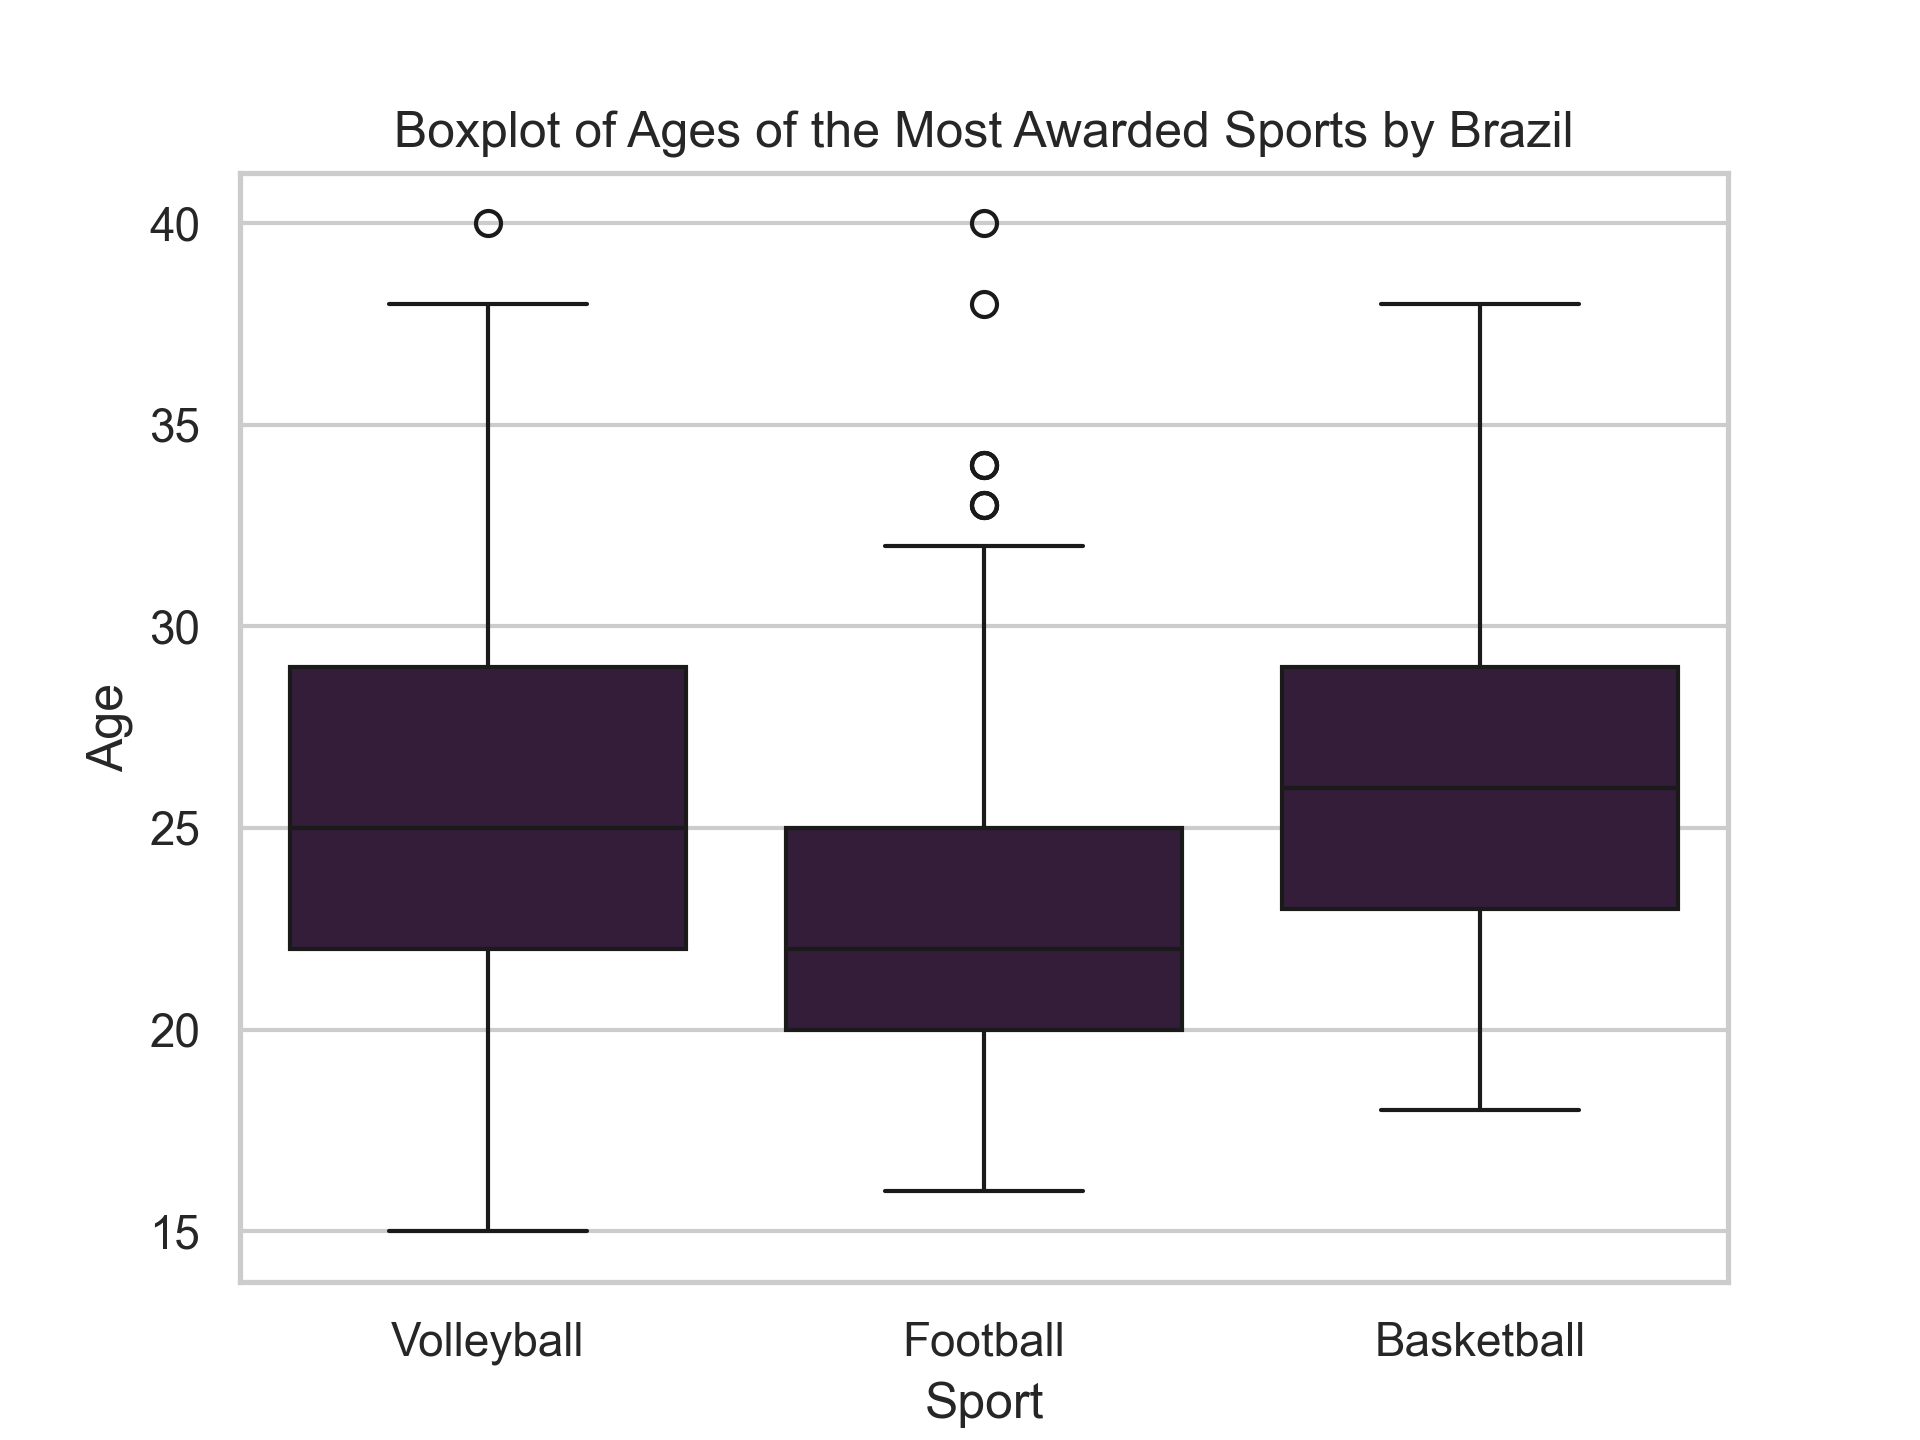
\includegraphics[width=0.5\textwidth]{images/age_analysis/boxplot_top_3_most_awarded.png}
\caption{\label{fig3}Boxplot with the Highest Amount of Brazilian Medalists}
\end{figure}

\subsection{Association of Physical Attributes with Medal Awards}
\paragraph{Observing the Data}
From this analysis, it is also possible to investigate the association between other physical variables and the medal outcomes for Brazilian athletes. Using a sample from the three sports in which Brazil has won the most medals, association tables were generated, considering both global and Brazilian data.

\begin{table}[h!]
    \centering
    \small
    \caption{Association between Age and Medal Awards by Sport and Region}
    \begin{tabular}{|c|c|c|}
        \hline
        \textbf{Sport} & \textbf{Region} & \textbf{Age-Medal Association} \\
        \hline
        Football   & World    & 0.0048 \\
        Football   & Brazil   & 0.0030 \\
        Volleyball & World    & 0.0085 \\
        Volleyball & Brazil   & 0.1200 \\
        Basketball & World    & $8.3 \times 10^{-6}$ \\
        Basketball & Brazil   & 0.0264 \\
        \hline
    \end{tabular}
\end{table}

\begin{table}[h!]
    \centering
    \small
    \caption{Association between Height and Medal Awards by Sport and Region}
    \begin{tabular}{|c|c|c|}
        \hline
        \textbf{Sport} & \textbf{Region} & \textbf{Height-Medal Association} \\
        \hline
        Football   & World    & $2.05 \times 10^{-5}$ \\
        Football   & Brazil   & 0.0500 \\
        Volleyball & World    & $5.99 \times 10^{-5}$ \\
        Volleyball & Brazil   & 0.0700 \\
        Basketball & World    & 0.0130 \\
        Basketball & Brazil   & 0.0500 \\
        \hline
    \end{tabular}
\end{table}

\begin{table}[h!]
    \centering
    \small
    \caption{Association between Weight and Medal Awards by Sport and Region}
    \begin{tabular}{|c|c|c|}
        \hline
        \textbf{Sport} & \textbf{Region} & \textbf{Weight-Medal Association} \\
        \hline
        Football   & World    & 0.0002 \\
        Football   & Brazil   & 0.0400 \\
        Volleyball & World    & 0.0009 \\
        Volleyball & Brazil   & 0.0300 \\
        Basketball & World    & 0.0007 \\
        Basketball & Brazil   & 0.0500 \\
        \hline
    \end{tabular}
\end{table}


From these results, it is evident that the association between physical characteristics and medal outcomes is quite limited across all sports. Although there is a slight association for Brazilian athletes in some cases, the overall impact remains minimal, with no clear pattern of physical attributes influencing medal performance in a consistent manner.

\begin{figure}[H]
    \centering
    \begin{subfigure}[b]{0.49\textwidth}
        \centering
        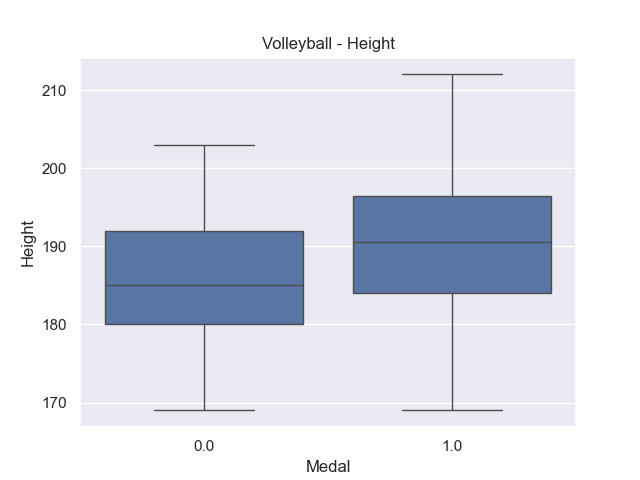
\includegraphics[width=\linewidth]{images/physical_attributes_graphs/Volleyball_Height.png} 
        \caption{Height}
        \label{fig:image1}
    \end{subfigure}
    \begin{subfigure}[b]{0.49\textwidth}
        \centering
        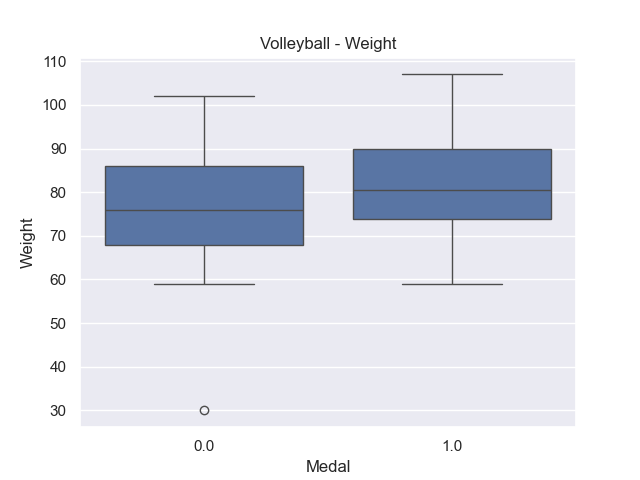
\includegraphics[width=\linewidth]{images/physical_attributes_graphs/Volleyball_Weight.png} 
        \caption{Weight}
        \label{fig:image2}
    \end{subfigure}
    \caption{Volleyball Athletes Physical Attributes Boxplot by Medal Status}
\end{figure}
\begin{figure}[H]
    \begin{subfigure}[b]{0.49\textwidth}
        \centering
        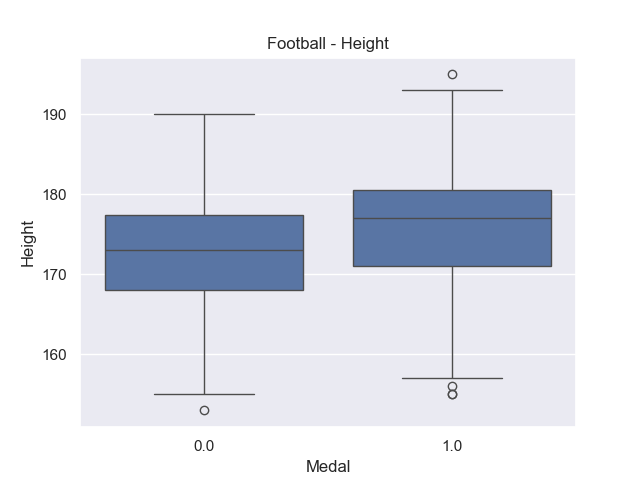
\includegraphics[width=\linewidth]{images/physical_attributes_graphs/Football_Height.png} 
        \caption{Height}
        \label{fig:image1}
    \end{subfigure}
    \begin{subfigure}[b]{0.49\textwidth}
        \centering
        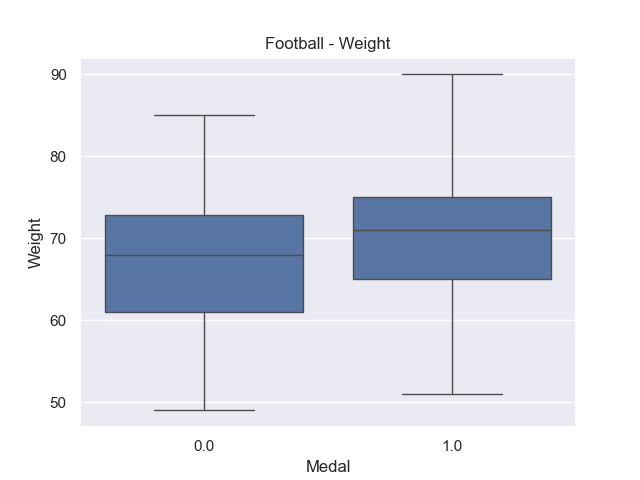
\includegraphics[width=\linewidth]{images/physical_attributes_graphs/Football_Weight.png}  
        \caption{Weight}
        \label{fig:image2}
    \end{subfigure}
    \caption{Football Athletes Physical Attributes Boxplot by Medal Status}
    
    \label{fig:sidebyside}
\end{figure}

\paragraph{Chronological Influence on Athletes' Physical Attributes}

Similarly, the chronological evolution of athletes' physical characteristics was investigated, focusing on how these attributes correlate with the year of the event. The following table summarizes the results for both global and Brazilian athletes.

\begin{table}[h!]
    \centering
    \caption{Correlation of Physical Attributes with Year by Region}
    \begin{tabular}{|c|c|c|}
        \hline
        \textbf{Attribute} & \textbf{Region} & \textbf{Year Correlation} \\
        \hline
        Age     & World   & -0.1247 \\
        Age     & Brazil  & 0.0451 \\
        Height  & World   & -0.0091 \\
        Height  & Brazil  & -0.1208 \\
        Weight  & World   & -0.0585 \\
        Weight  & Brazil  & -0.1355 \\
        \hline
    \end{tabular}
\end{table}

Among the physical attributes, age demonstrates the strongest correlation with the event year, although this correlation remains weak. For Brazilian athletes, there was practically no variation in age over the years. However, both height and weight showed a slightly more significant correlation with the year of the event, compared to age, though the association is still of low magnitude.


\subsection{Female Participation Analysis}

Athletes were also categorized by gender to assess whether the presence and performance of male and female athletes have become more balanced over time. This analysis seeks to identify potential disparities in participation and outcomes between the two groups, contributing to a deeper understanding of gender dynamics in Olympic competitions.

With our scoring system, it became possible to compare the performances of both genders on a global scale and within Brazil. It is important to note that the analysis includes both Summer and Winter Olympic Games, which may result in significant differences in the number of athletes between seasons. However, despite these variations, an increase in performance for both genders was observed over time.

\begin{figure}[h]
    \centering
    \begin{subfigure}[b]{0.49\textwidth}
        \centering
        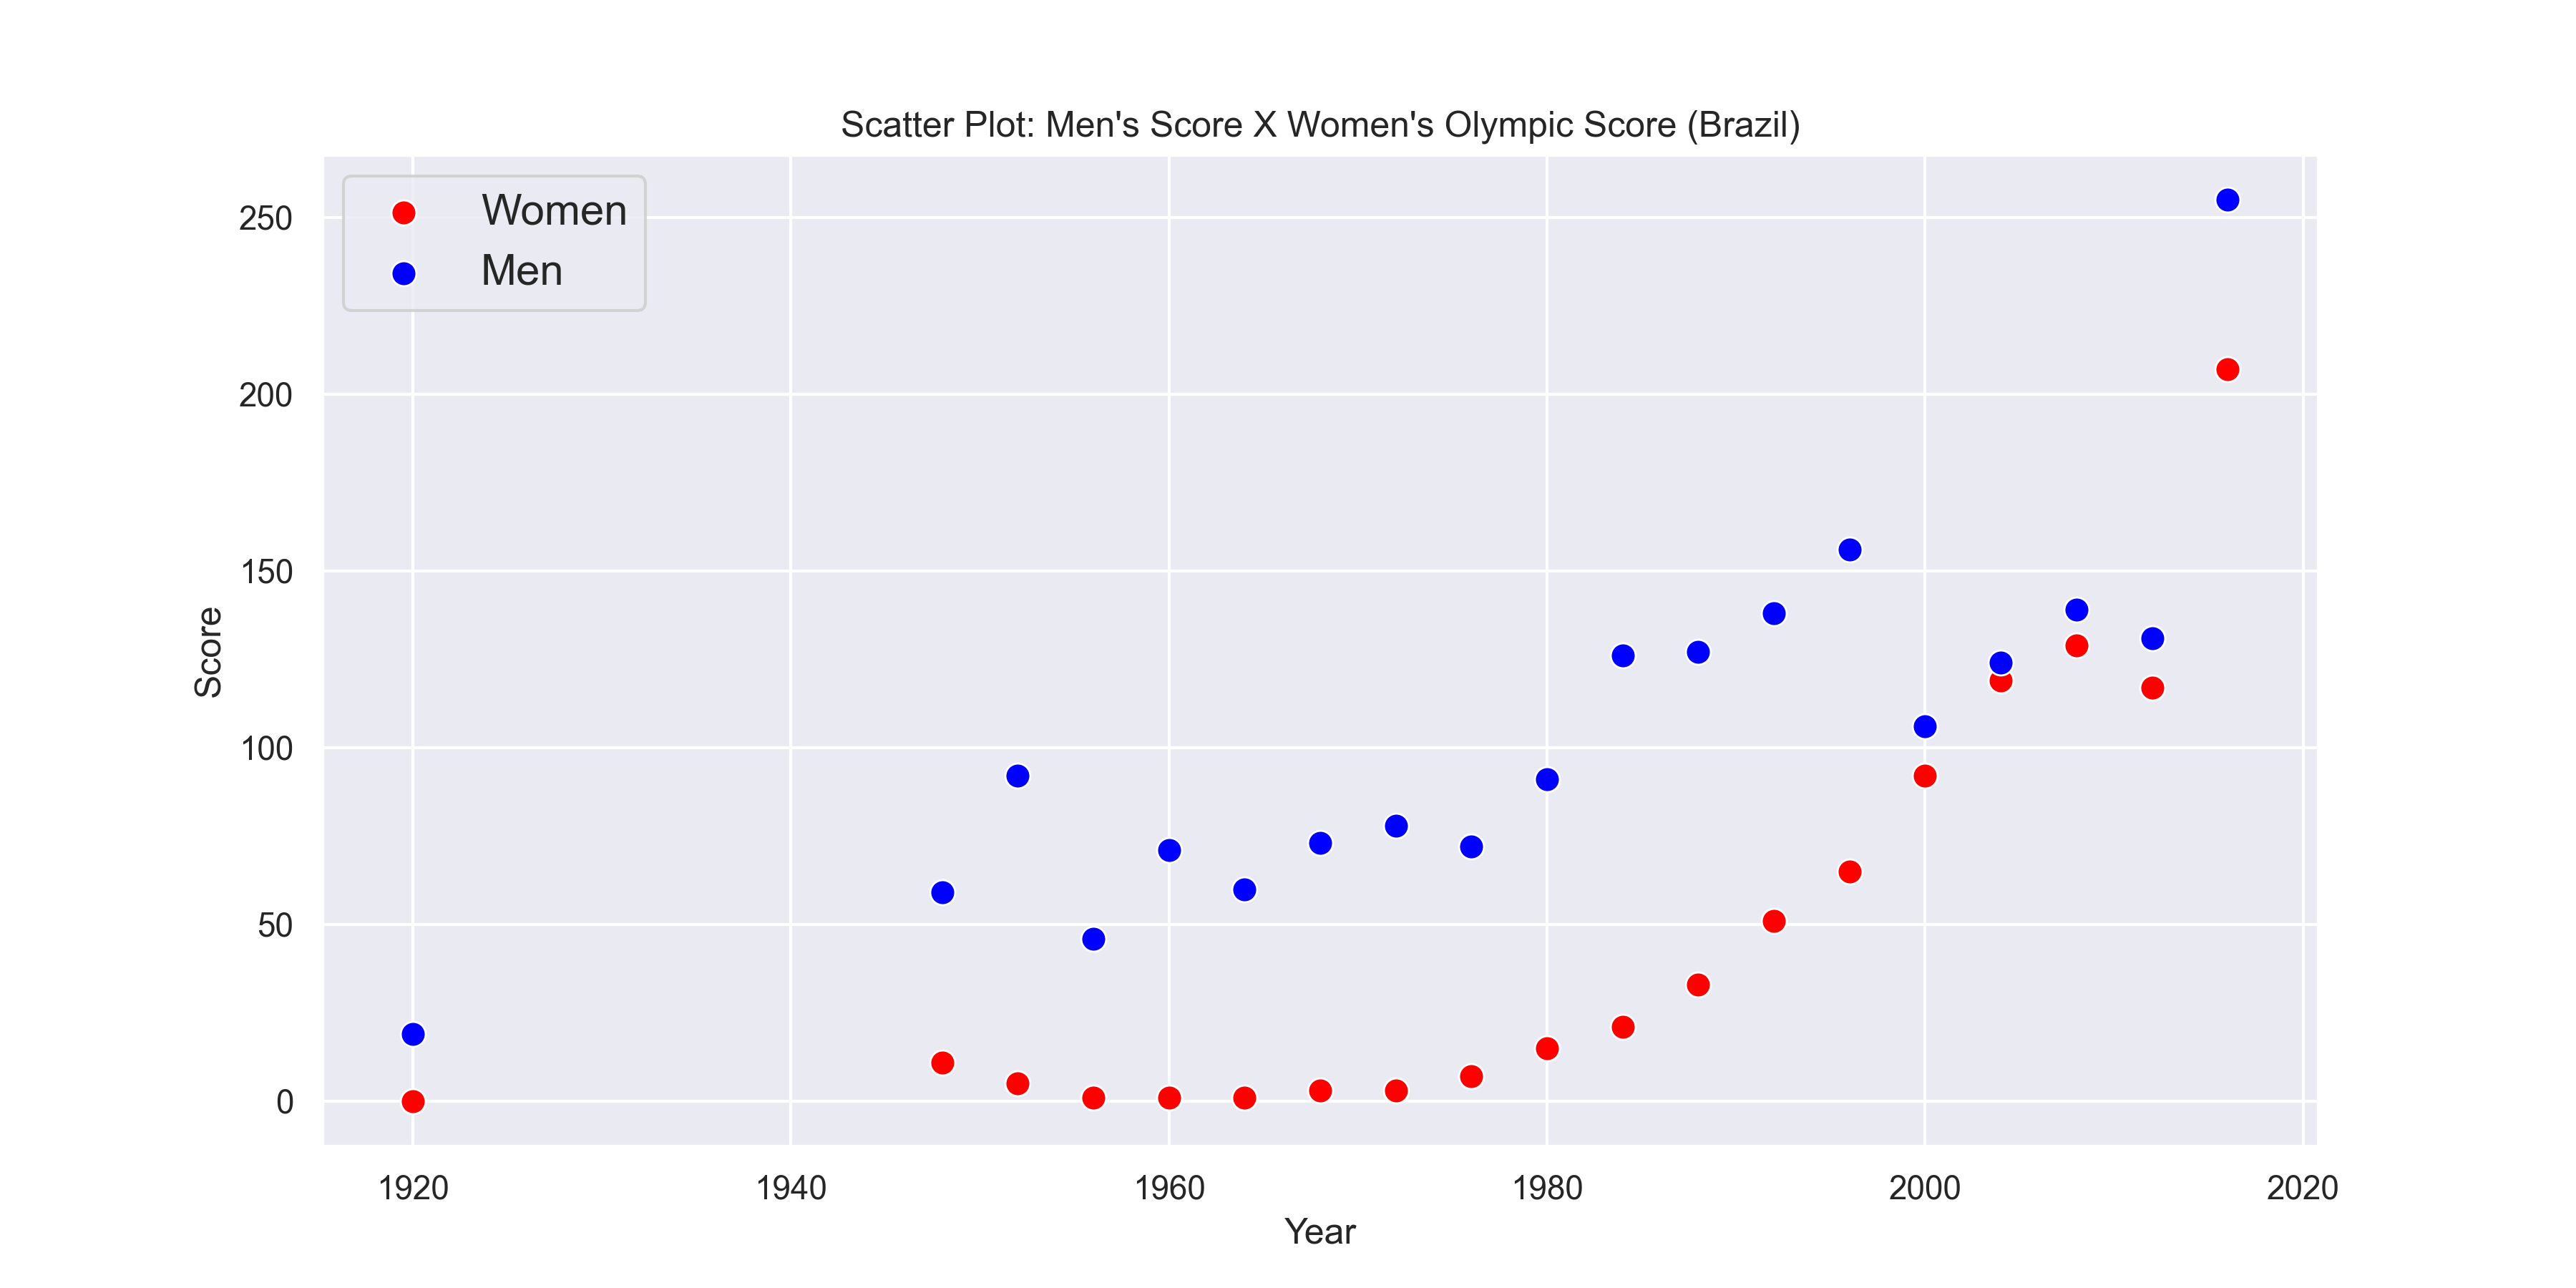
\includegraphics[width=\linewidth]{images/female_participation/scatterplot_olymp_score_bra.png} 
        \caption{Brazil}
        \label{fig:image1}
    \end{subfigure}
    \begin{subfigure}[b]{0.49\textwidth}
        \centering
        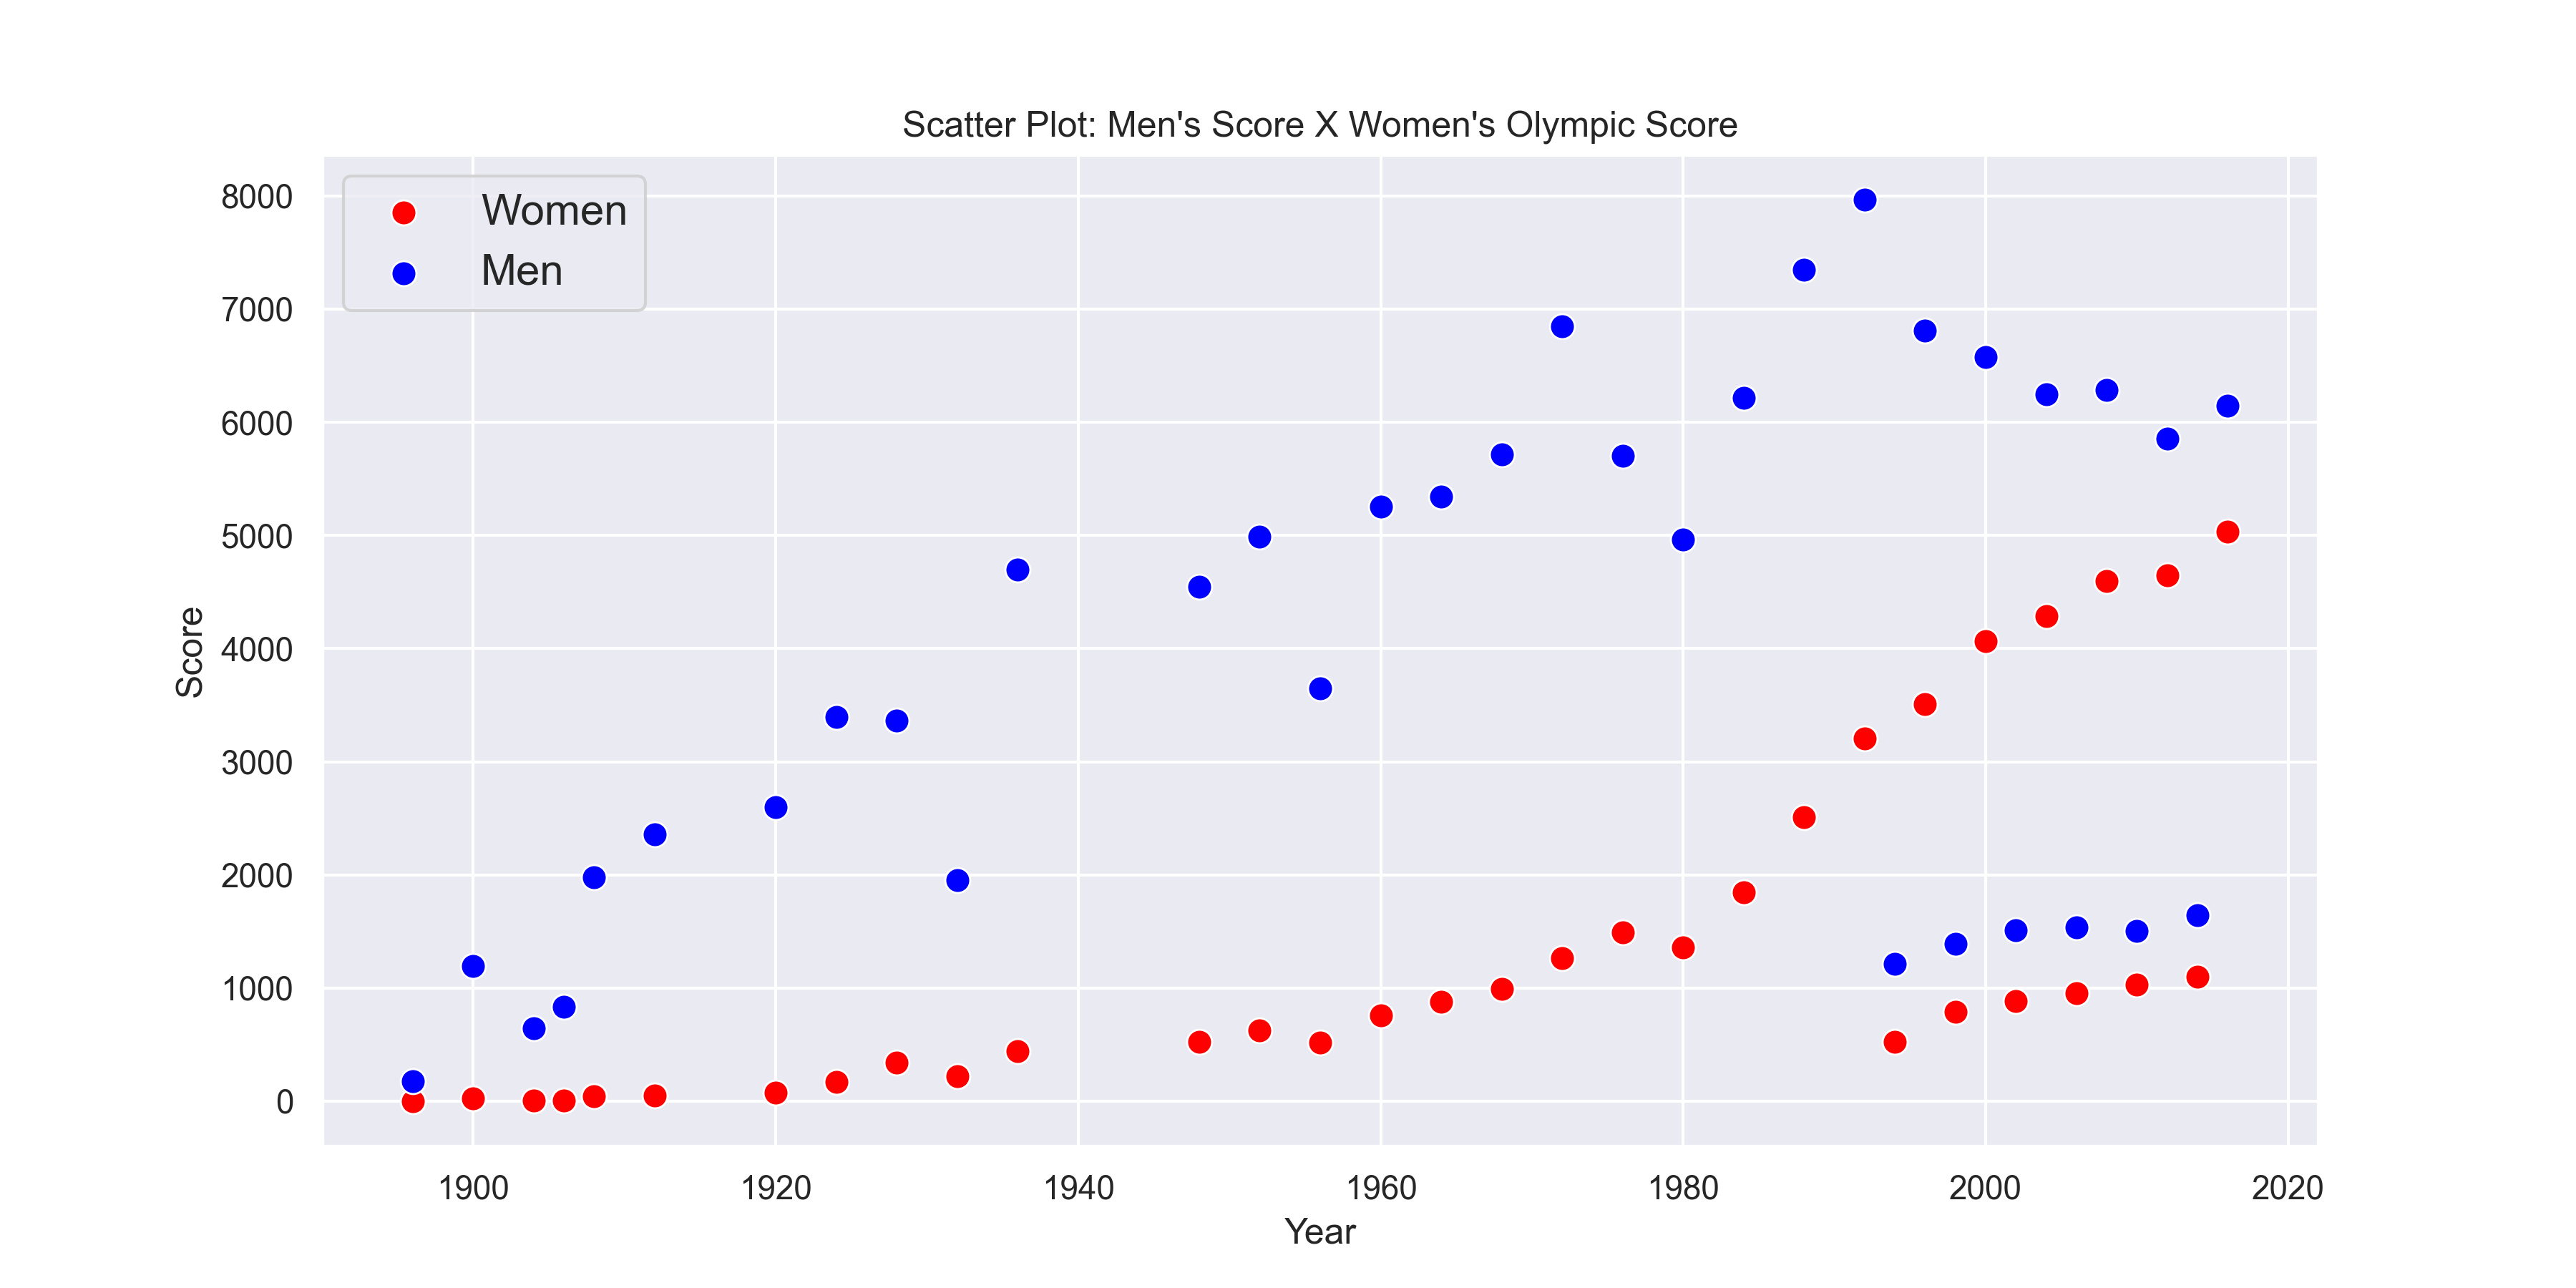
\includegraphics[width=\linewidth]{images/female_participation/scatterplot_olymp_score_global.png} 
        \caption{Global}
        \label{fig:image2}
    \end{subfigure}
    \caption{Score calculated as the sum of weighted medals (Gold: 3, Silver: 2, Bronze: 1)}
    \label{fig:sidebyside}
\end{figure}

When analyzing the scatterplots of the Paralympic Games, the global trend mirrors that of the Olympic Games. However, when comparing the Brazilian Olympic and Paralympic trends, we notice that while the Olympic curve shows steady growth, the Paralympic trend fluctuates, rising and falling several times. Globally, female performance in both the Olympics and Paralympics seems to improve over time with fewer fluctuations. This trend does not hold in Brazil, where, in the Olympics, female performance declines between 2000 and 2020—a pattern not reflected globally. In the Paralympics, Brazilian female performance appears inversely correlated to the global trend around the 1990s and 2012, suggesting no clear relationship.

\begin{figure}[H]
    \centering
    \begin{subfigure}[b]{0.49\textwidth}
        \centering
        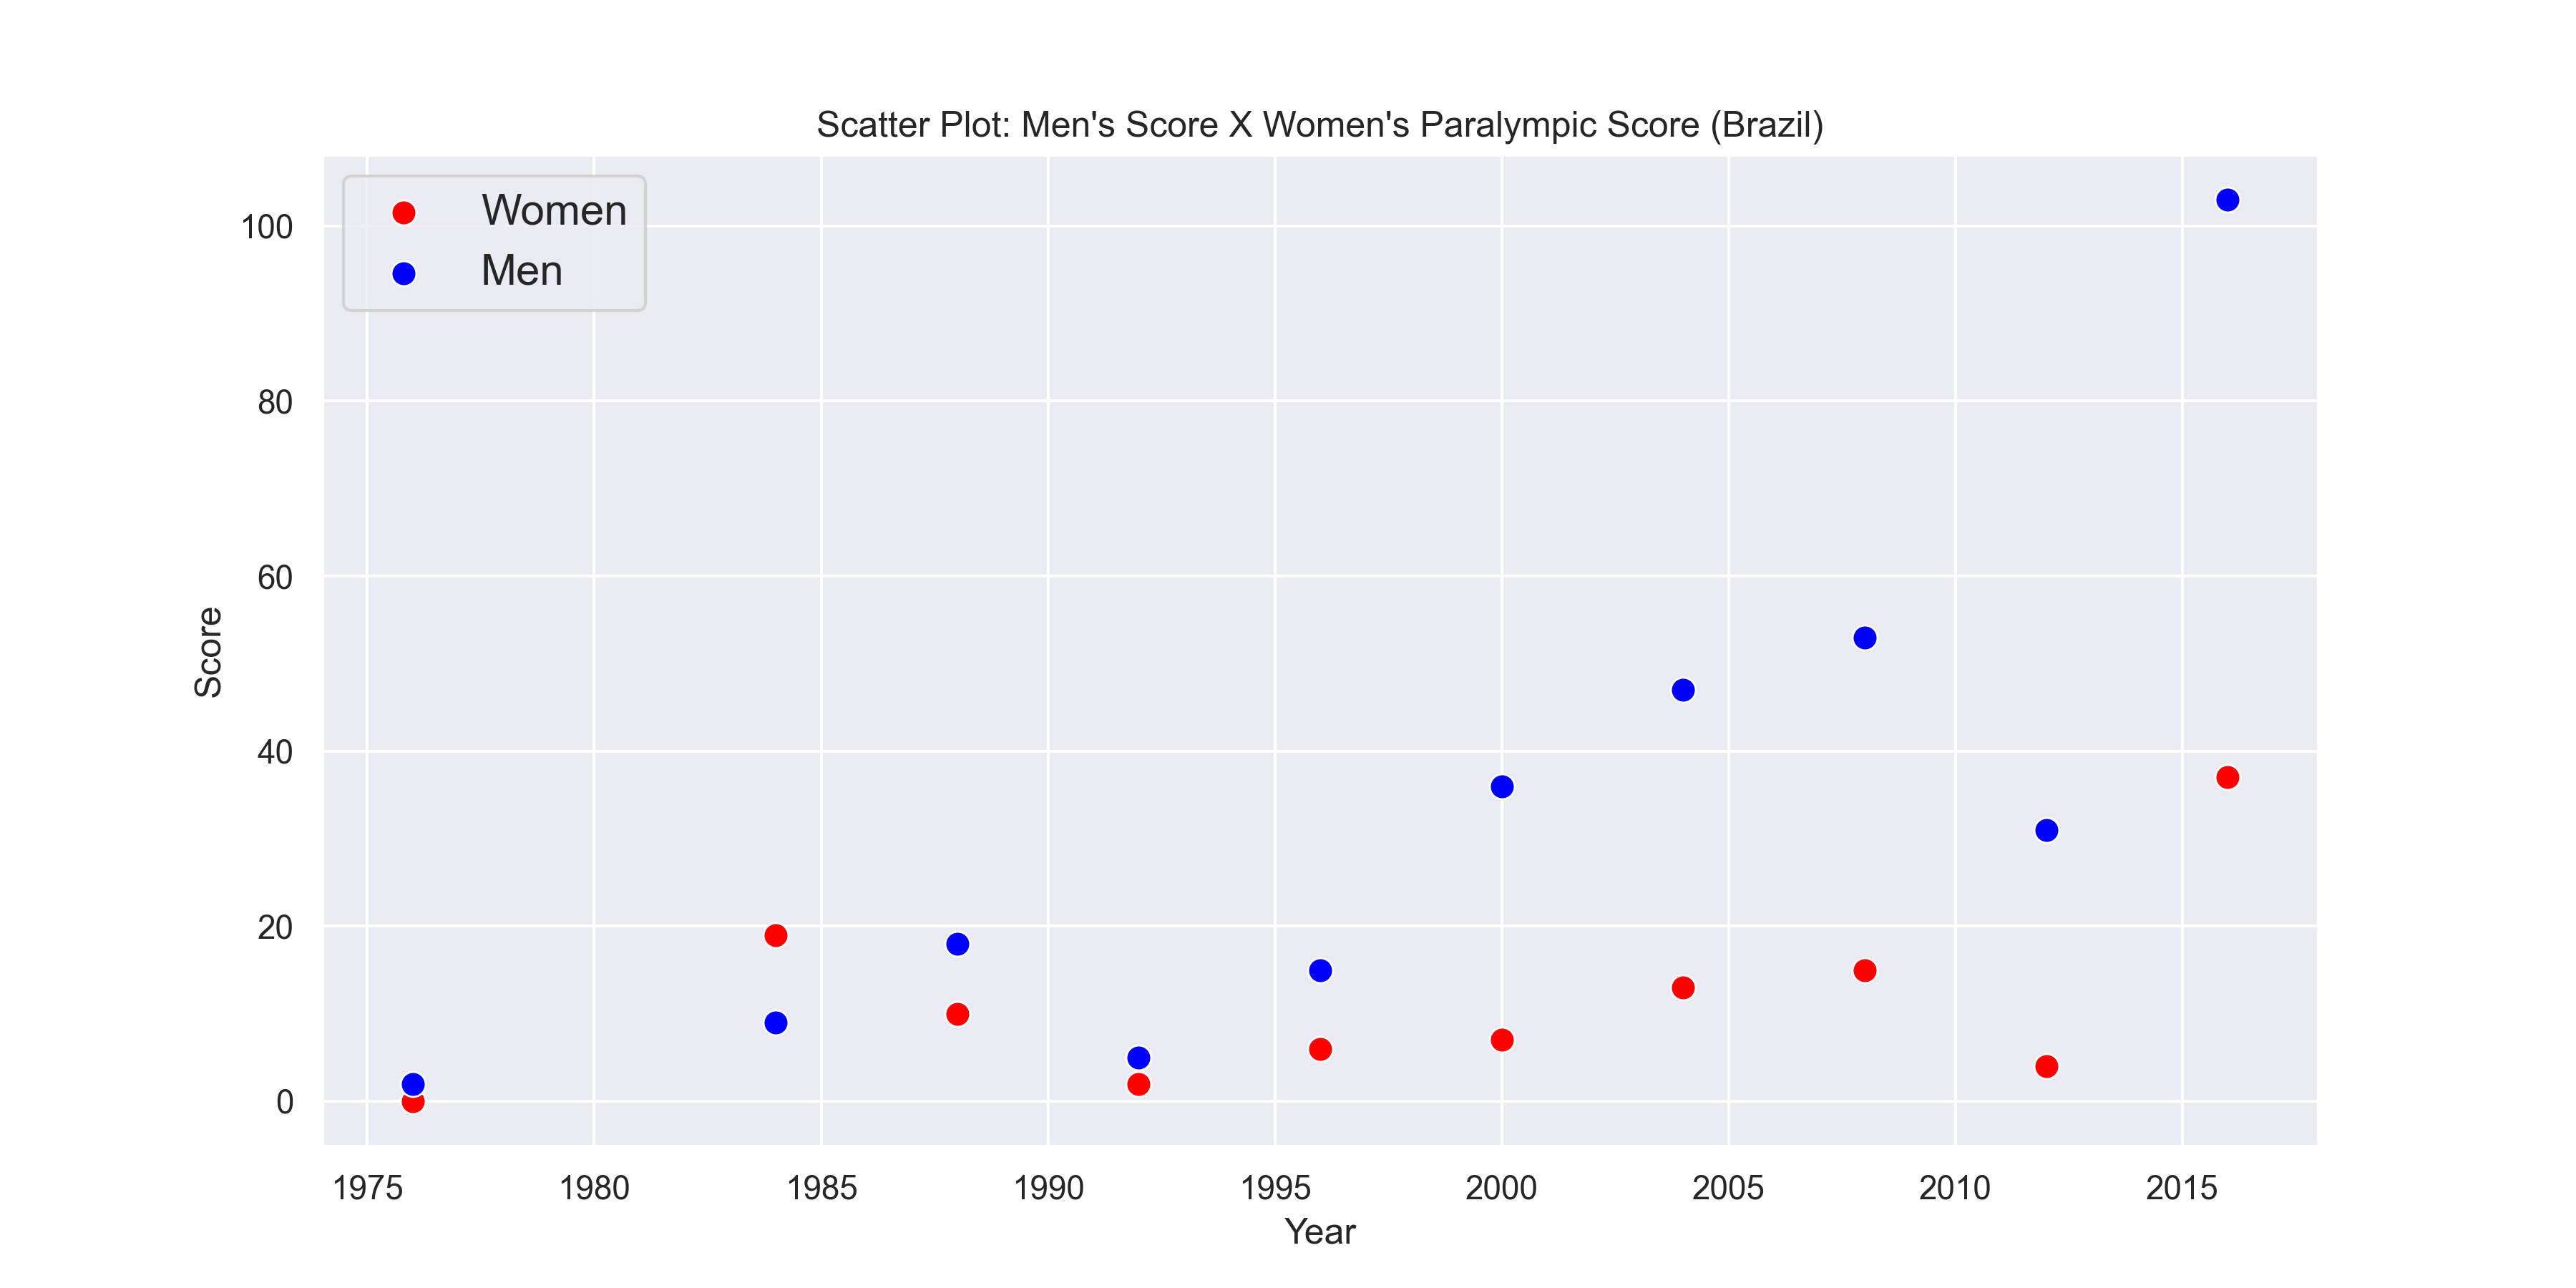
\includegraphics[width=\linewidth]{images/female_participation/scatterplot_paralymp_score_bra.png} 
        \caption{Brazil}
        \label{fig:image1}
    \end{subfigure}
    \begin{subfigure}[b]{0.49\textwidth}
        \centering
        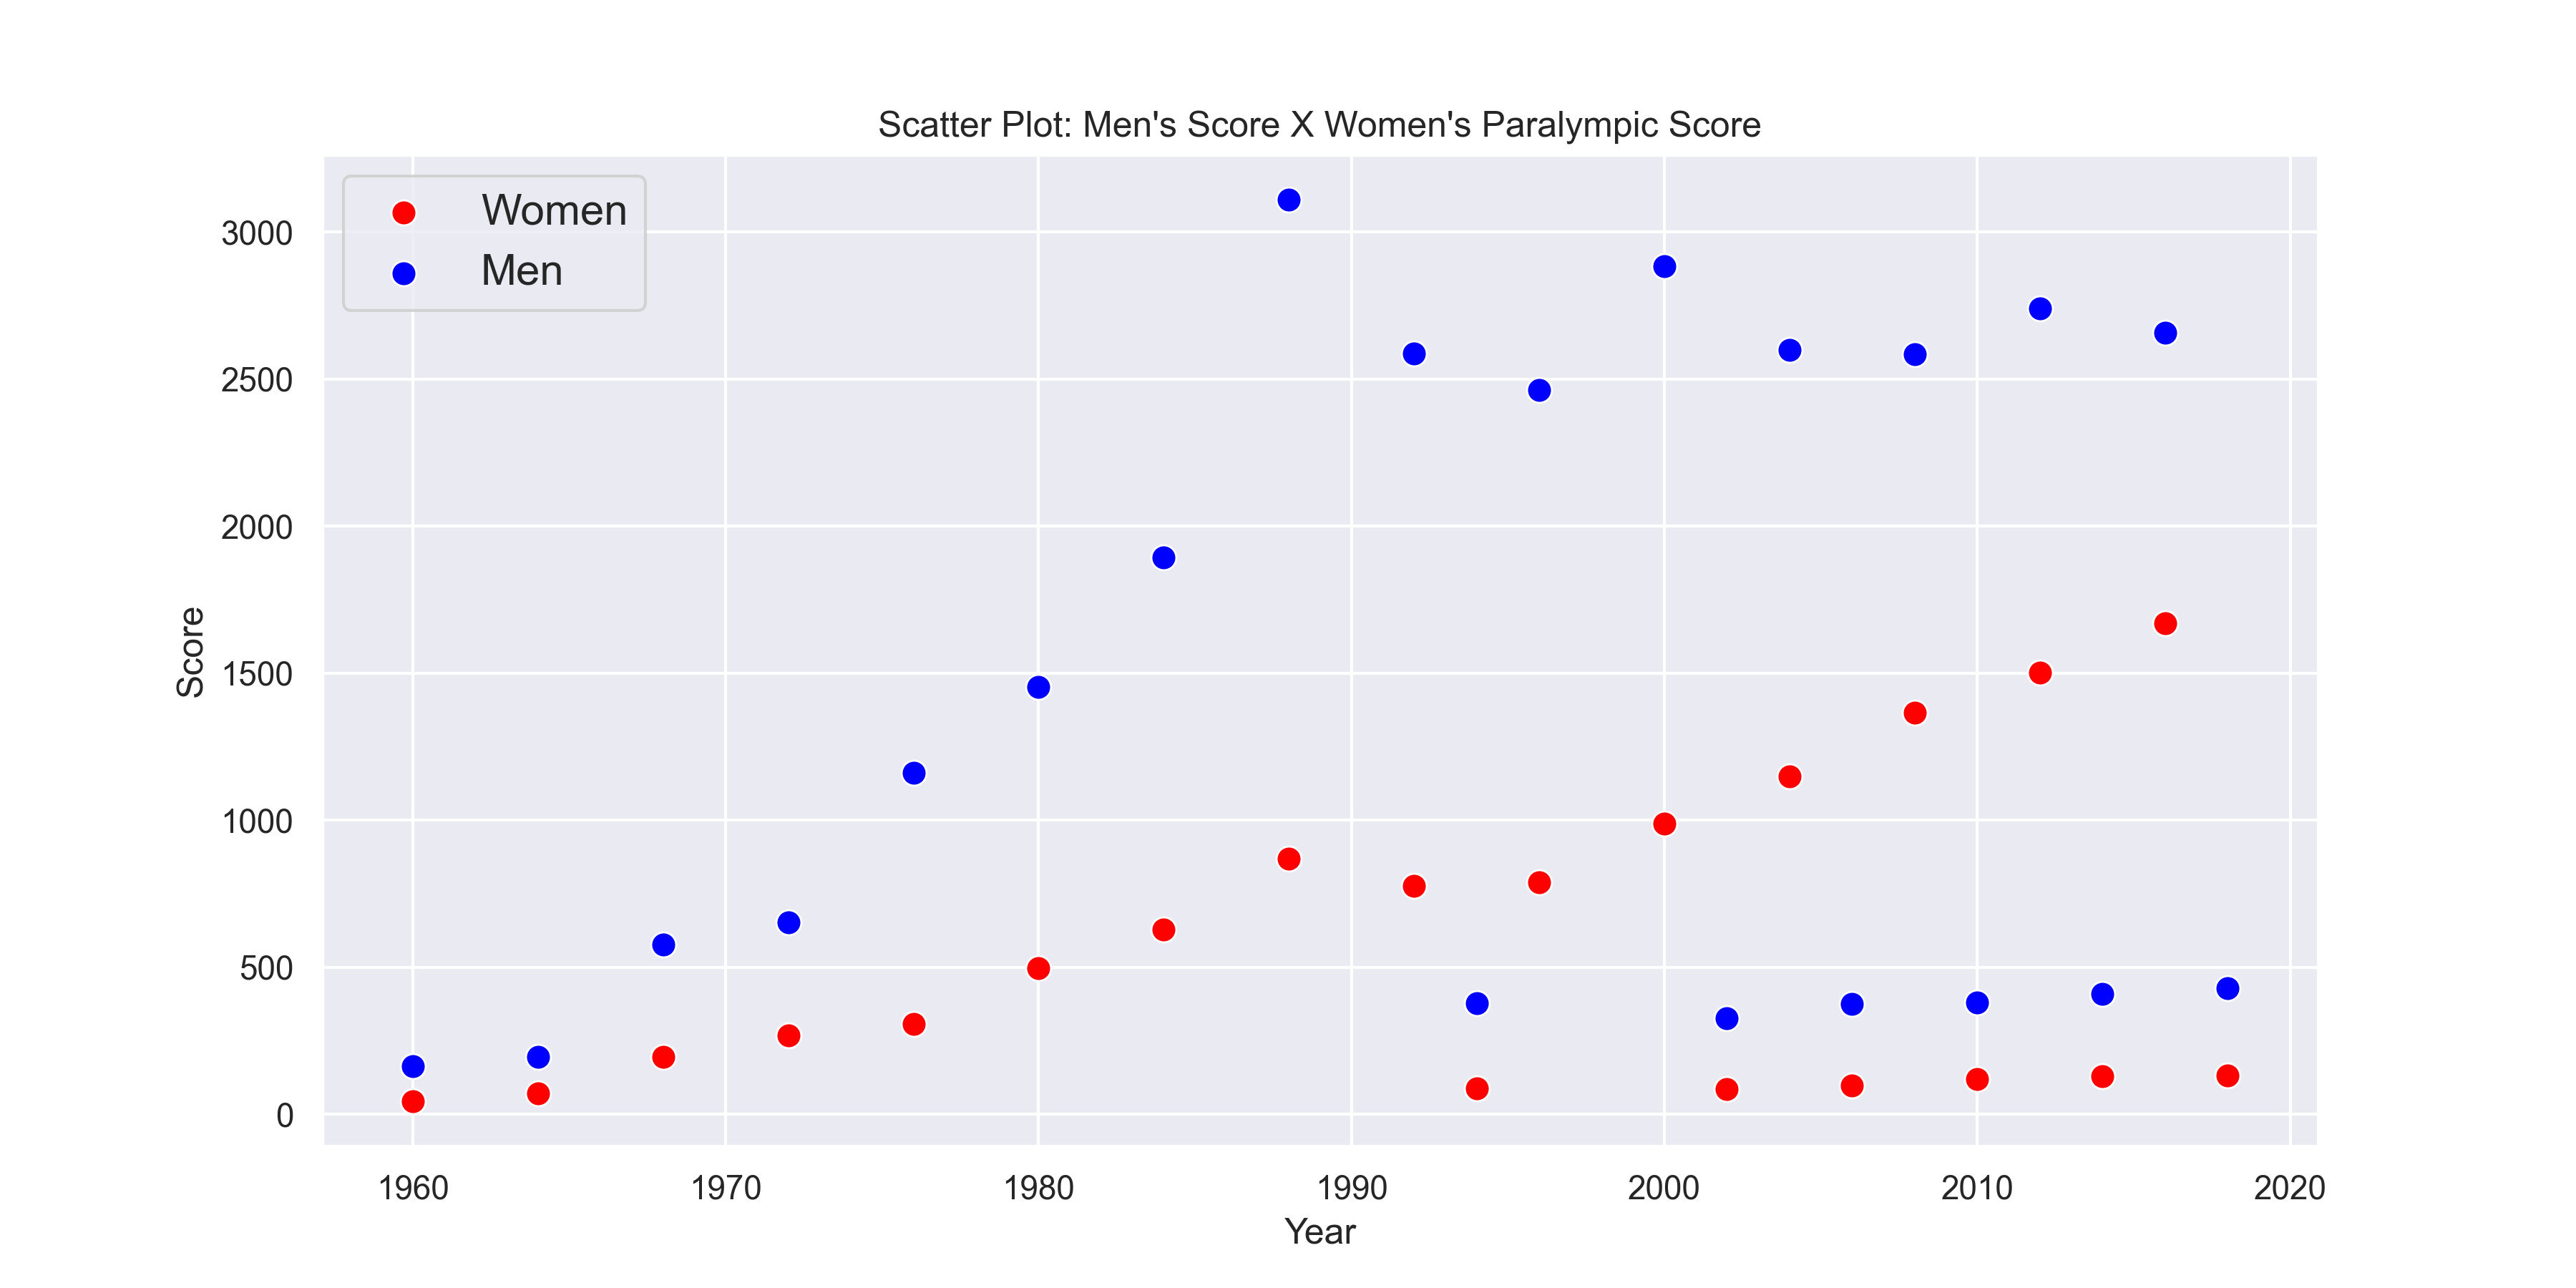
\includegraphics[width=\linewidth]{images/female_participation/scatterplot_paralymp_score_global.png} 
        \caption{Global}
        \label{fig:image2}
    \end{subfigure}
    \caption{Score calculated as the sum of weighted medals (Gold: 3, Silver: 2, Bronze: 1)}
    \label{fig:sidebyside}
\end{figure}

Using data on the number of female athletes, medals won by women, and their performance in the Olympic and Paralympic Games for Brazil, we calculated the standard deviation of each variable using both raw data (Normal) and cleaned data, where cases with zero values for F\_Athletes, F\_Medal, and F\_Score were excluded (Cleaned). The analysis revealed that the standard deviation of performance and athlete numbers is higher for the Olympic athletes compared to the Paralympic athletes. However, the standard deviation of medal counts is greater for Paralympic athletes than Olympic athletes, highlighting the differences in performance between the two groups.

\begin{figure}[H]
\centering
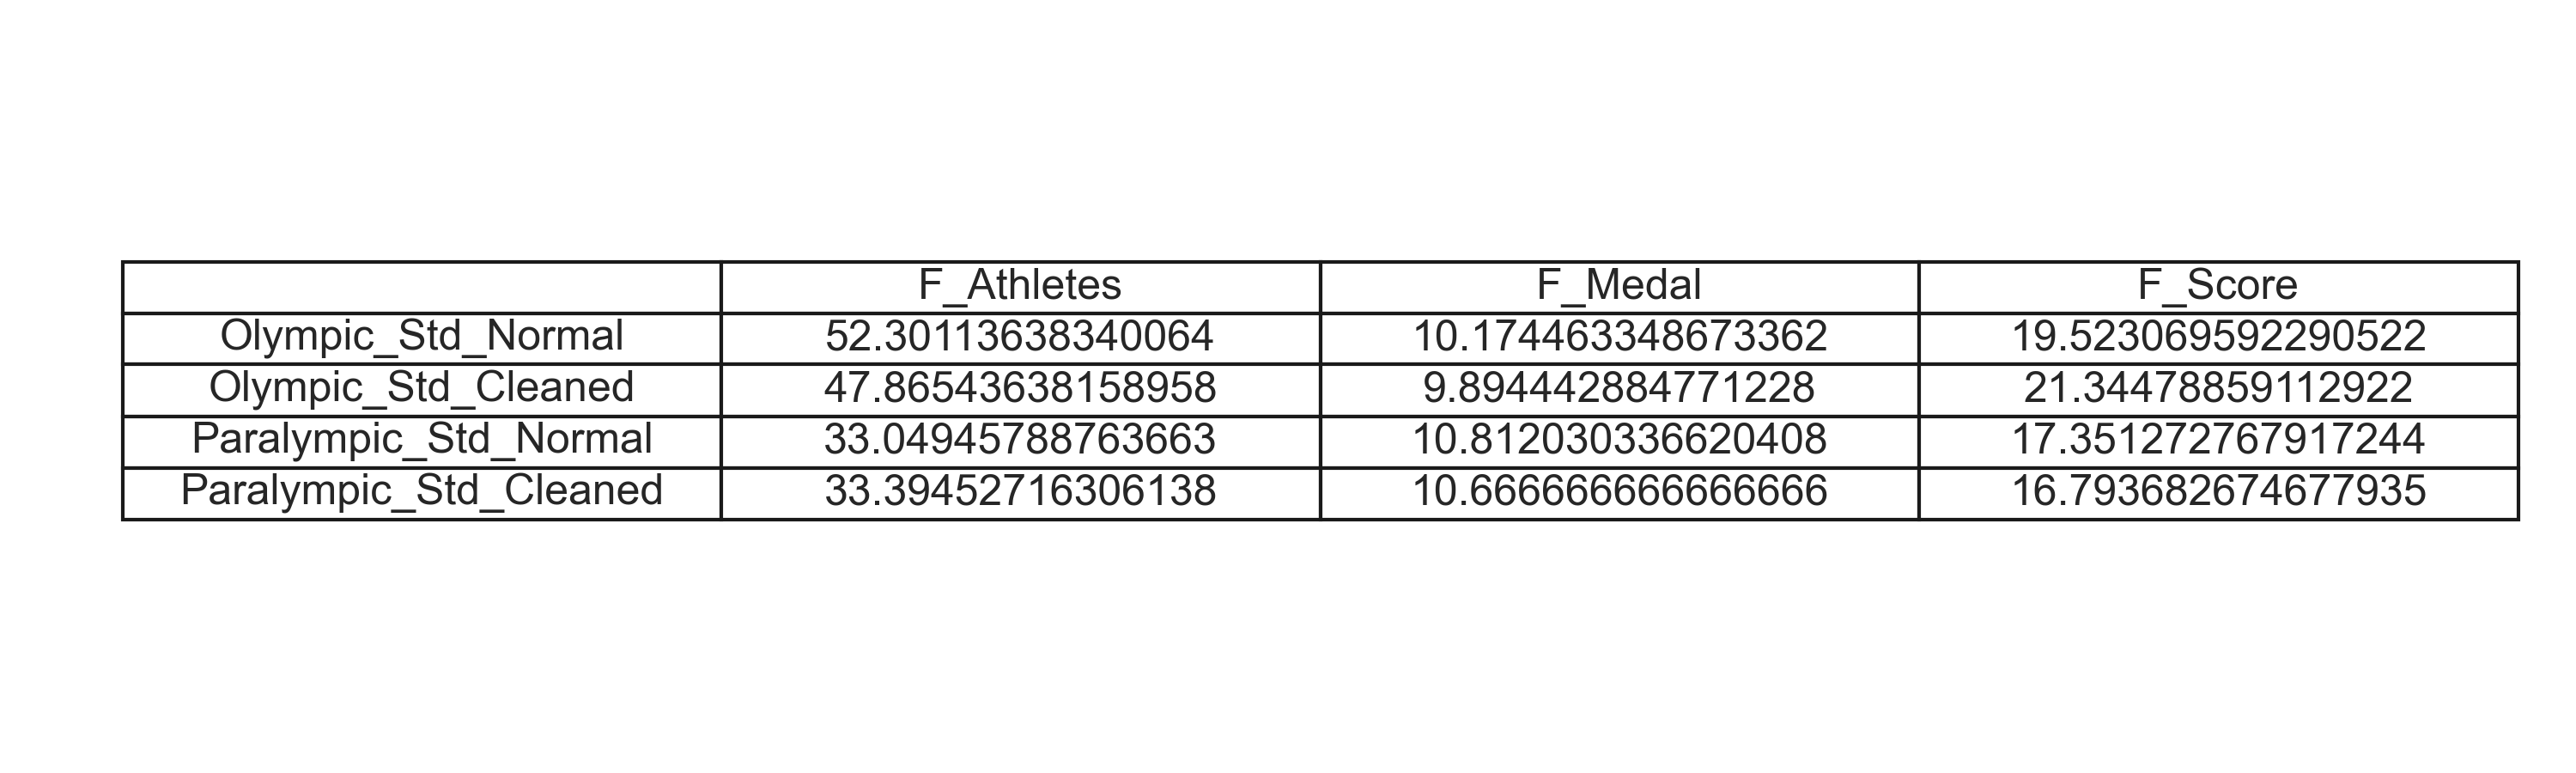
\includegraphics[width=1\textwidth]{images/female_participation/table_stds_olympics_and_paralympics_bra.png}
\caption{\label{fig5}Data Table for Brazilian Female Athletes}
\end{figure}

Therefore, to adequately address the original hypothesis, we need to differentiate between Olympic and Paralympic performance, as both exhibit entirely distinct patterns. While female performance in the Olympics shows a clear upward trend, Paralympic performance is more unstable, likely due to the difference in the number of athletes participating in Summer and Winter events. In the case of the Olympics, we can conclude that there has been an improvement in female athletes' performance over time. However, for the Paralympics, the current analysis does not provide sufficient evidence to draw a definitive conclusion.

\subsection{Urban Development Analysis}
\paragraph{Medalist Density per Urban Inhabitant}
In addition to considering individual factors within the sports modalities, we also included external factors such as the level of urbanization in the participating countries. 

We were able to conduct an initial analysis for the last available year, evaluating the density of medals per urban inhabitant and the percentage of the urban population in each country participating in the Olympics that year.

\begin{figure}[H]
\centering
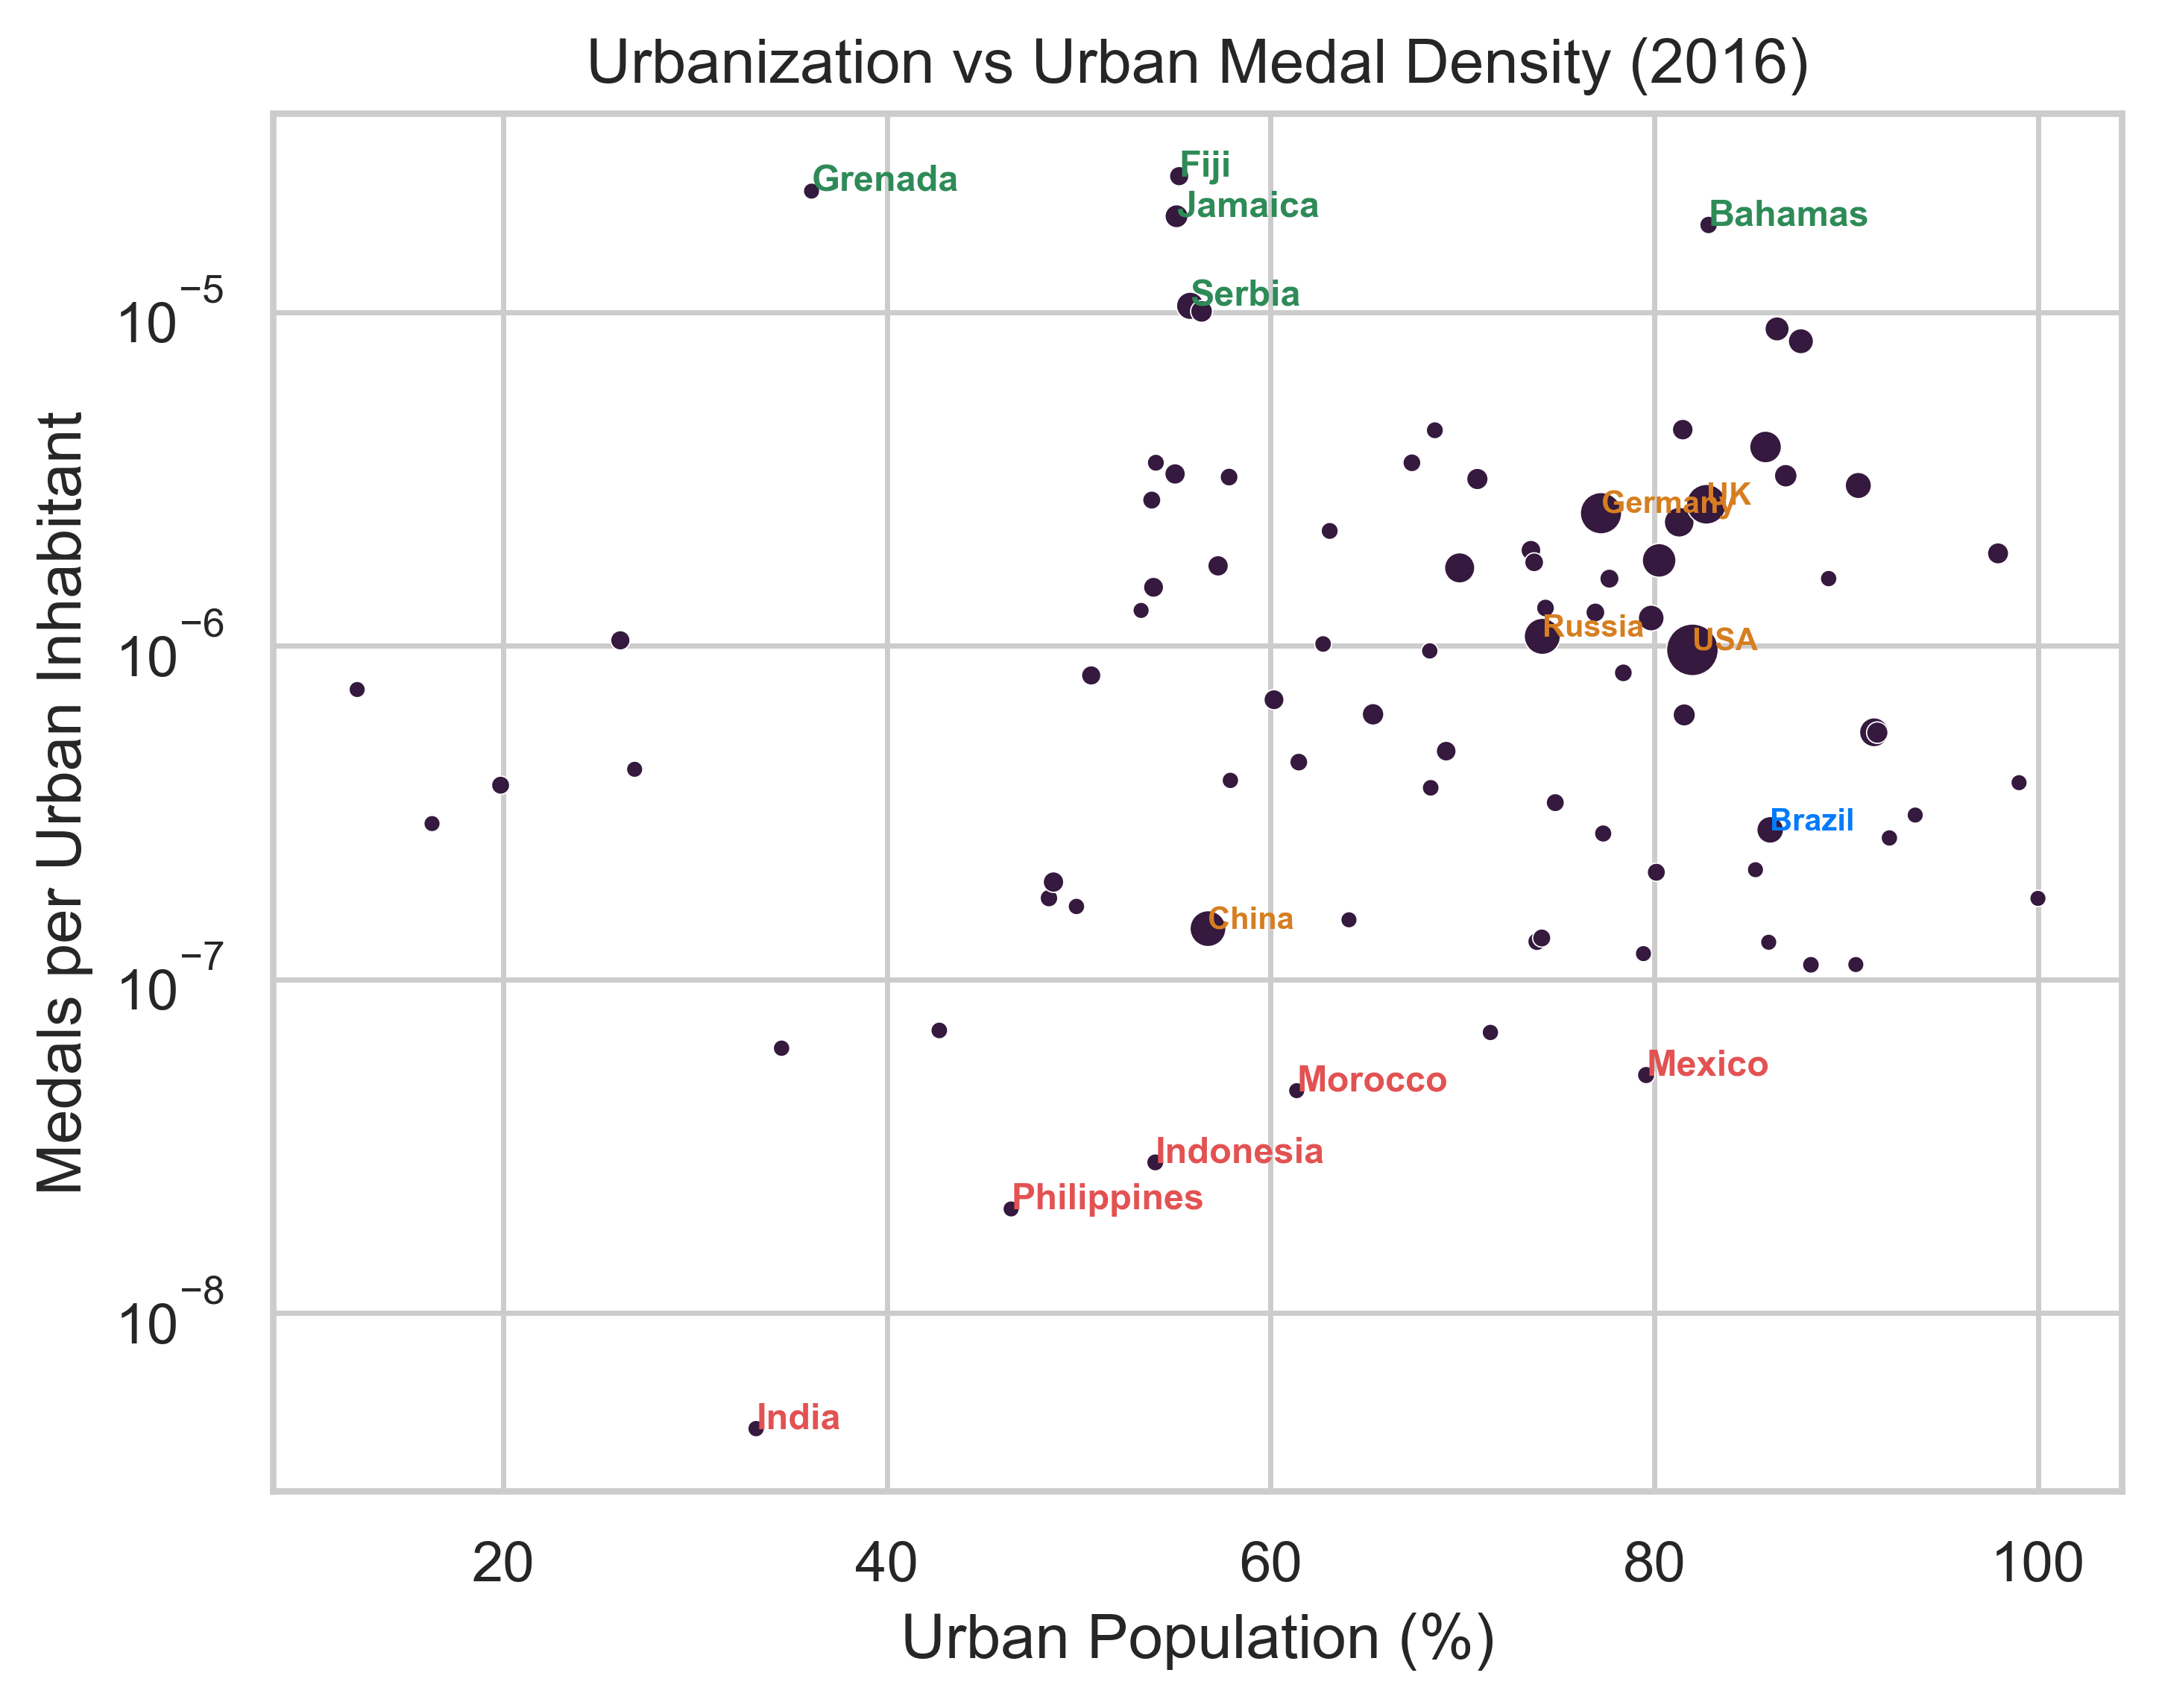
\includegraphics[width=0.75\textwidth]{images/urban/urban_medal_density.png}
\caption{\label{fig3}Scatterplot of Urban Development X Medal Density by Urban Inhabitant}
\end{figure}

It is expected to see countries with low populations and a reasonable amount of medals towards the top of the graph (e.g. Bahamas and Fiji), as their low population lifts the Medal Density. In contrast, it is also expected to observe high population countries heading towards the lower end of the graph (e. g. India and Indonesia). An interesting case is China, which, despite having an amount of medals comparable to countries such as Russia and the United Kingdom, stayed way beneath the other top medalists countries (marked in yellow) due to the sheer magnitude of its population.
\paragraph{Growth Over Time}
Regarding the temporal evolution of countries concerning these variables—such as medal density per urban inhabitant and urban population percentage—we were also able to analyze which countries experienced synchronized growth or decline in these factors.

\begin{figure}[H]
\centering
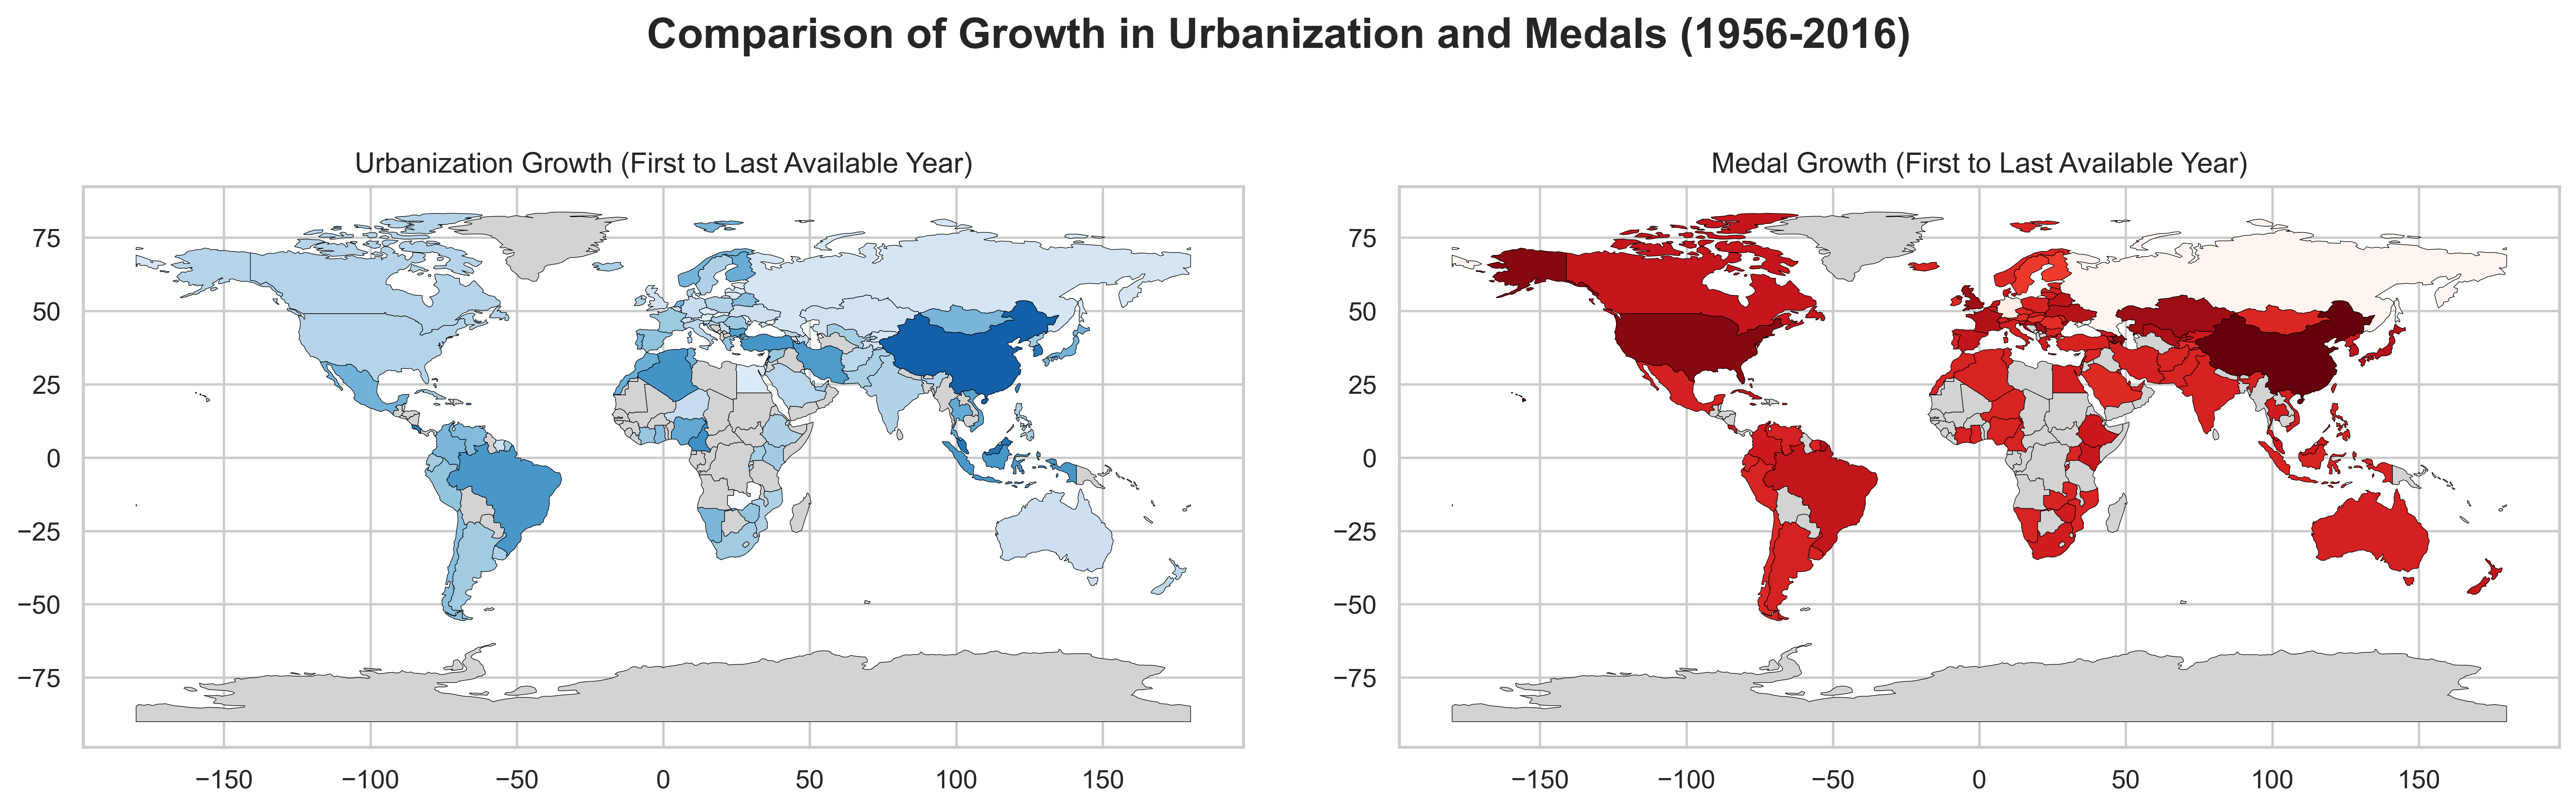
\includegraphics[width=1\textwidth]{images/urban/geographic_growth.png}
\caption{\label{fig3}Geographic Visualization for Urban and Medal Growth}
\end{figure}

\[Growth_X = \frac{X_2 - X_1}{Y_2 - Y_1} \]
Where $X_2 - X_1$ is the difference between the Urbanization Percentages|Amount of Medals for the last and first available year for each country, respectively; and $Y_2 - Y_1$ is the difference between the last and first available years.

A comparison of urbanization trends and medal counts suggests a potential link between urban growth and athletic success. China and Brazil, for instance, saw increases in both categories. Conversely, highly urbanized nations like the United States, Canada, and many European countries experienced rising medal counts without significant urbanization changes. Germany, however, provides a counterexample: despite urban growth since its reunification in 1990, its medal count has been in decline each year. The previous examples highlight the nuanced relationship between these factors and how different contexts may impact the relationship between urbanization and athletic performance.

\subsection{Economic Influence on Olympic and Paralympic Performance}

To further investigate the relationship between external factors and the performance of countries in the Olympic and Paralympic Games, a dataset containing information on Gross Domestic Product (GDP) was incorporated. This addition aimed to understand whether economic conditions can influence athletic success.

After organizing and cleaning the data, the analysis initially focused on the correlation between the number of medals won in the Olympic and Paralympic Games. It also explored the relationship between the total number of medals won and the GDP of each country. A strong correlation was observed between Olympic and Paralympic performance, suggesting that countries performing well in one tend to excel in the other, likely due to investments in sports and related infrastructure. However, the correlation between the total medal count and GDP was moderate, indicating that factors beyond economic strength, such as sports policies and athlete support, play a role in success.

\begin{figure}[h]
    \centering
    \begin{subfigure}[b]{0.45\textwidth}
        \centering
        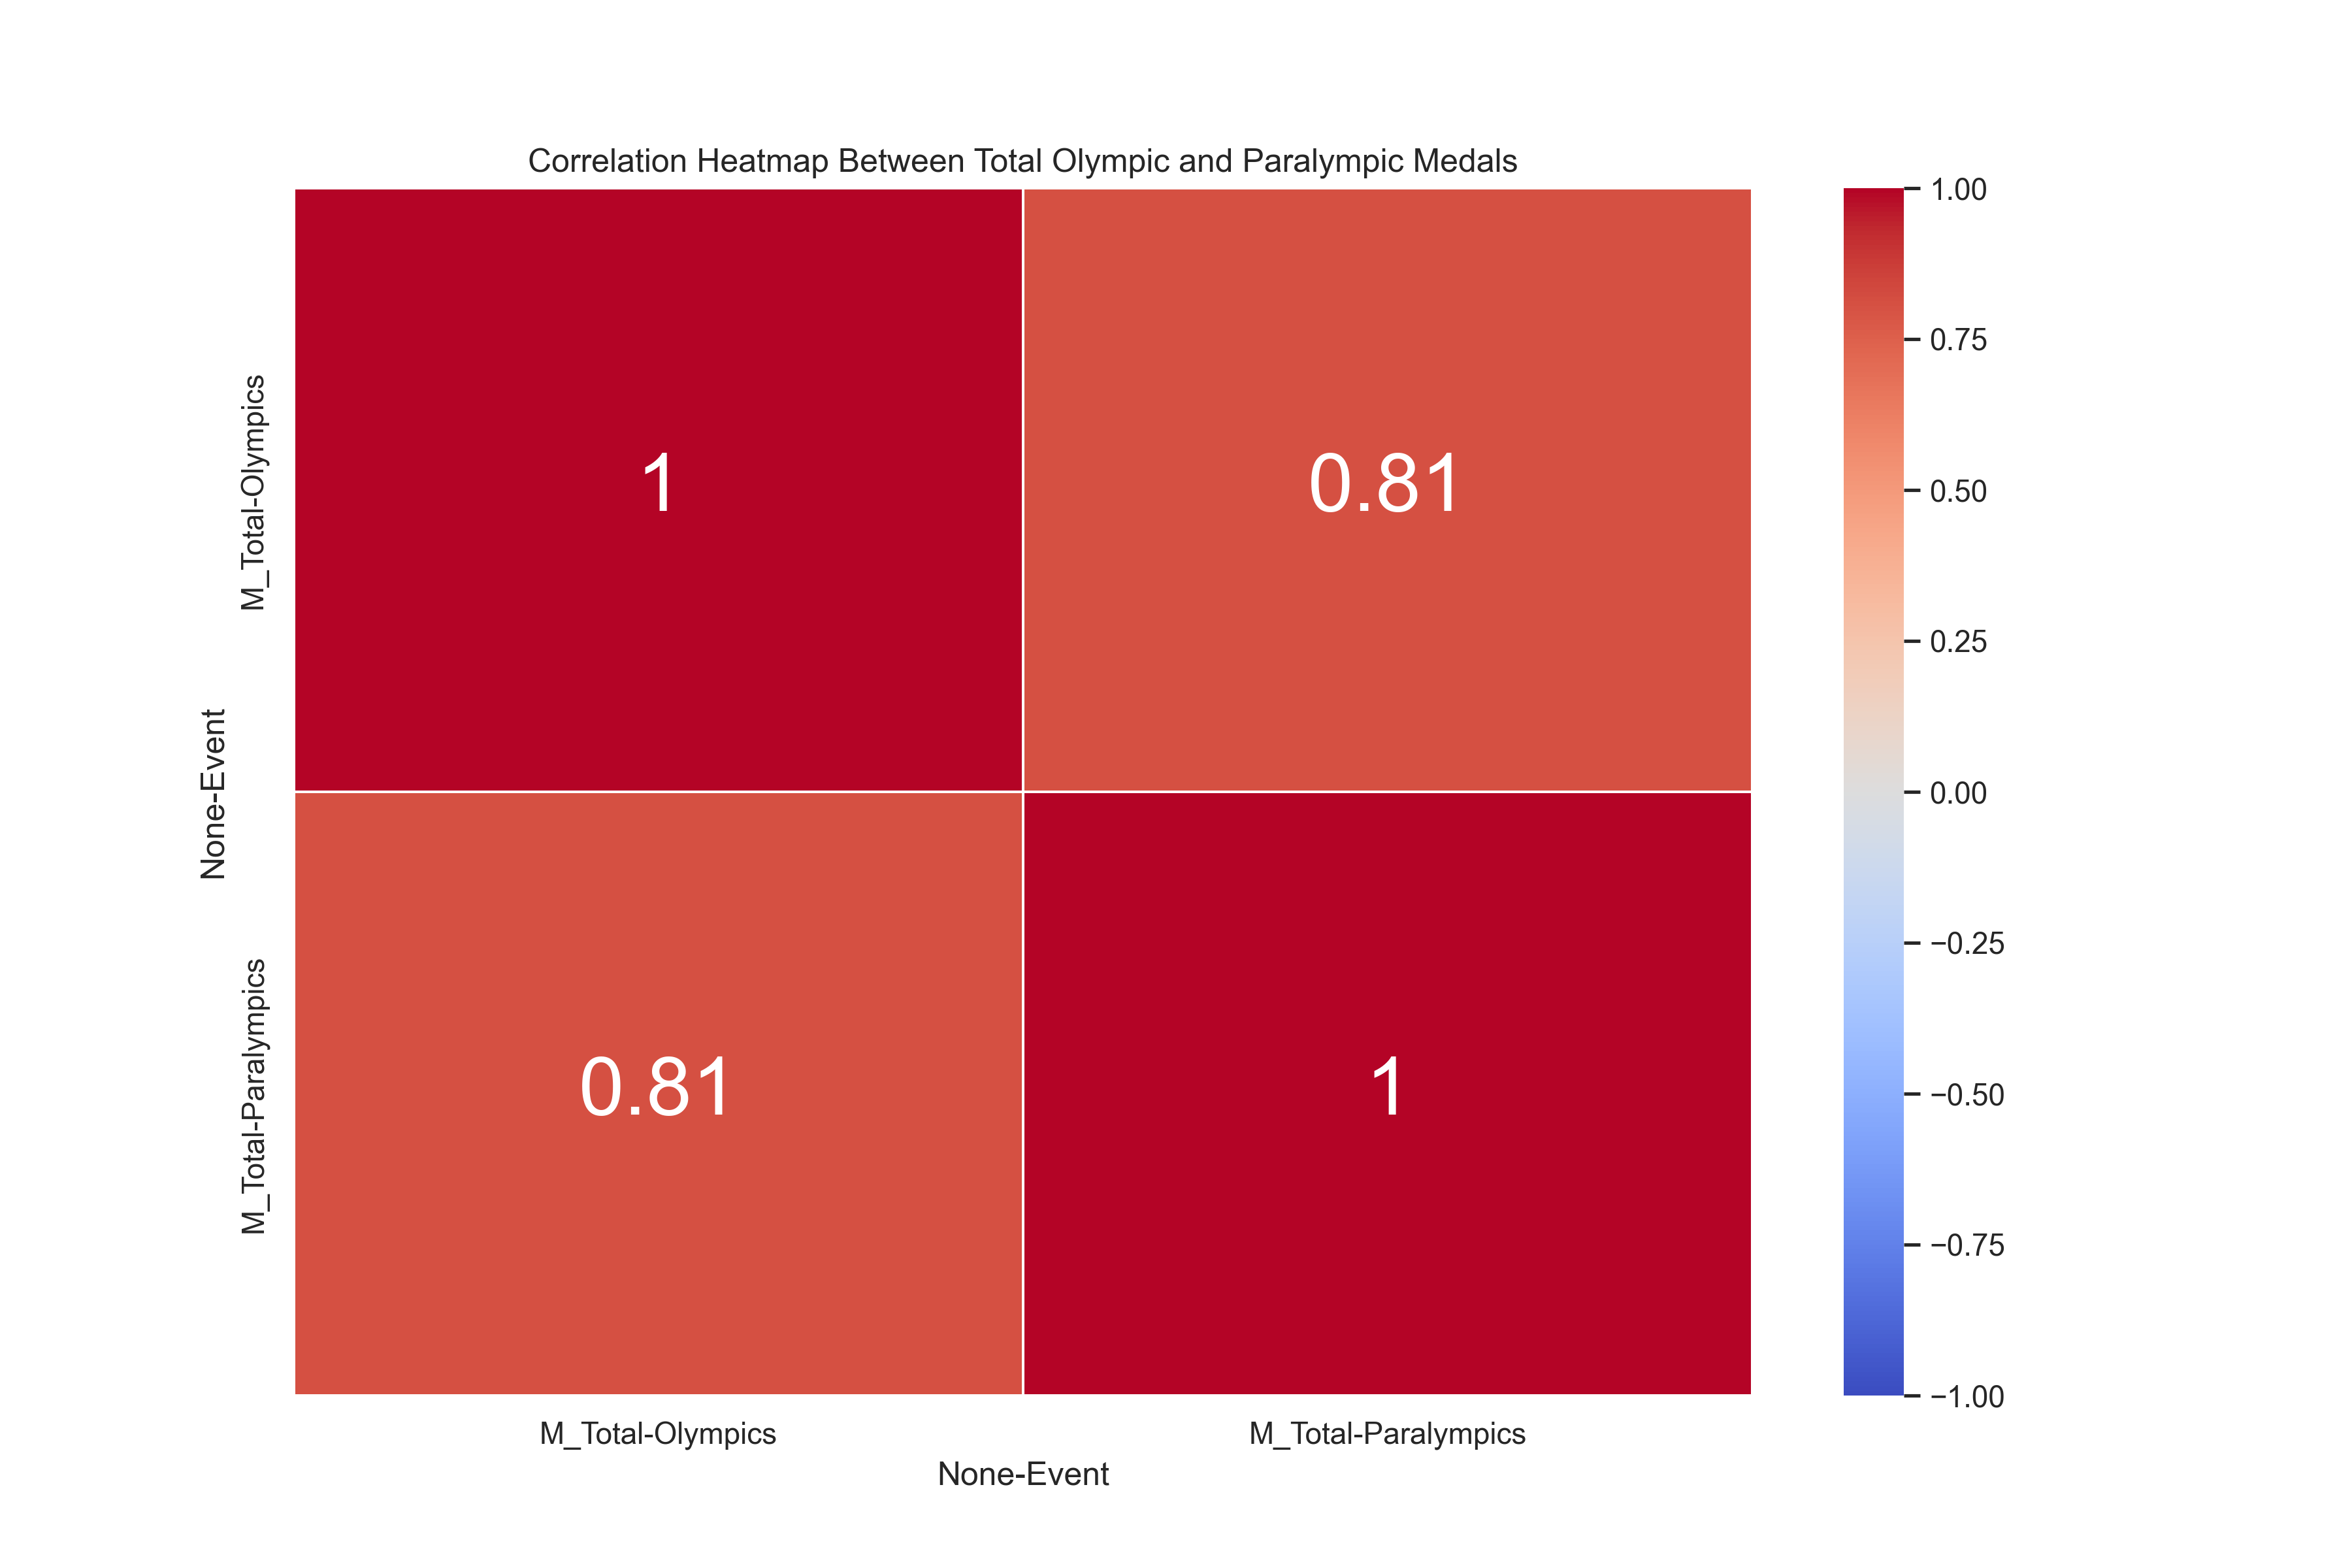
\includegraphics[width=\linewidth]{images/gdp_analysis/heatmap_olympics_paralympics_medals.png}
        \caption{Correlation between Olympic and Paralympic Performance}
        \label{fig:olympic_paralympic_corr}
    \end{subfigure}
    \hfill
    \begin{subfigure}[b]{0.45\textwidth}
        \centering
        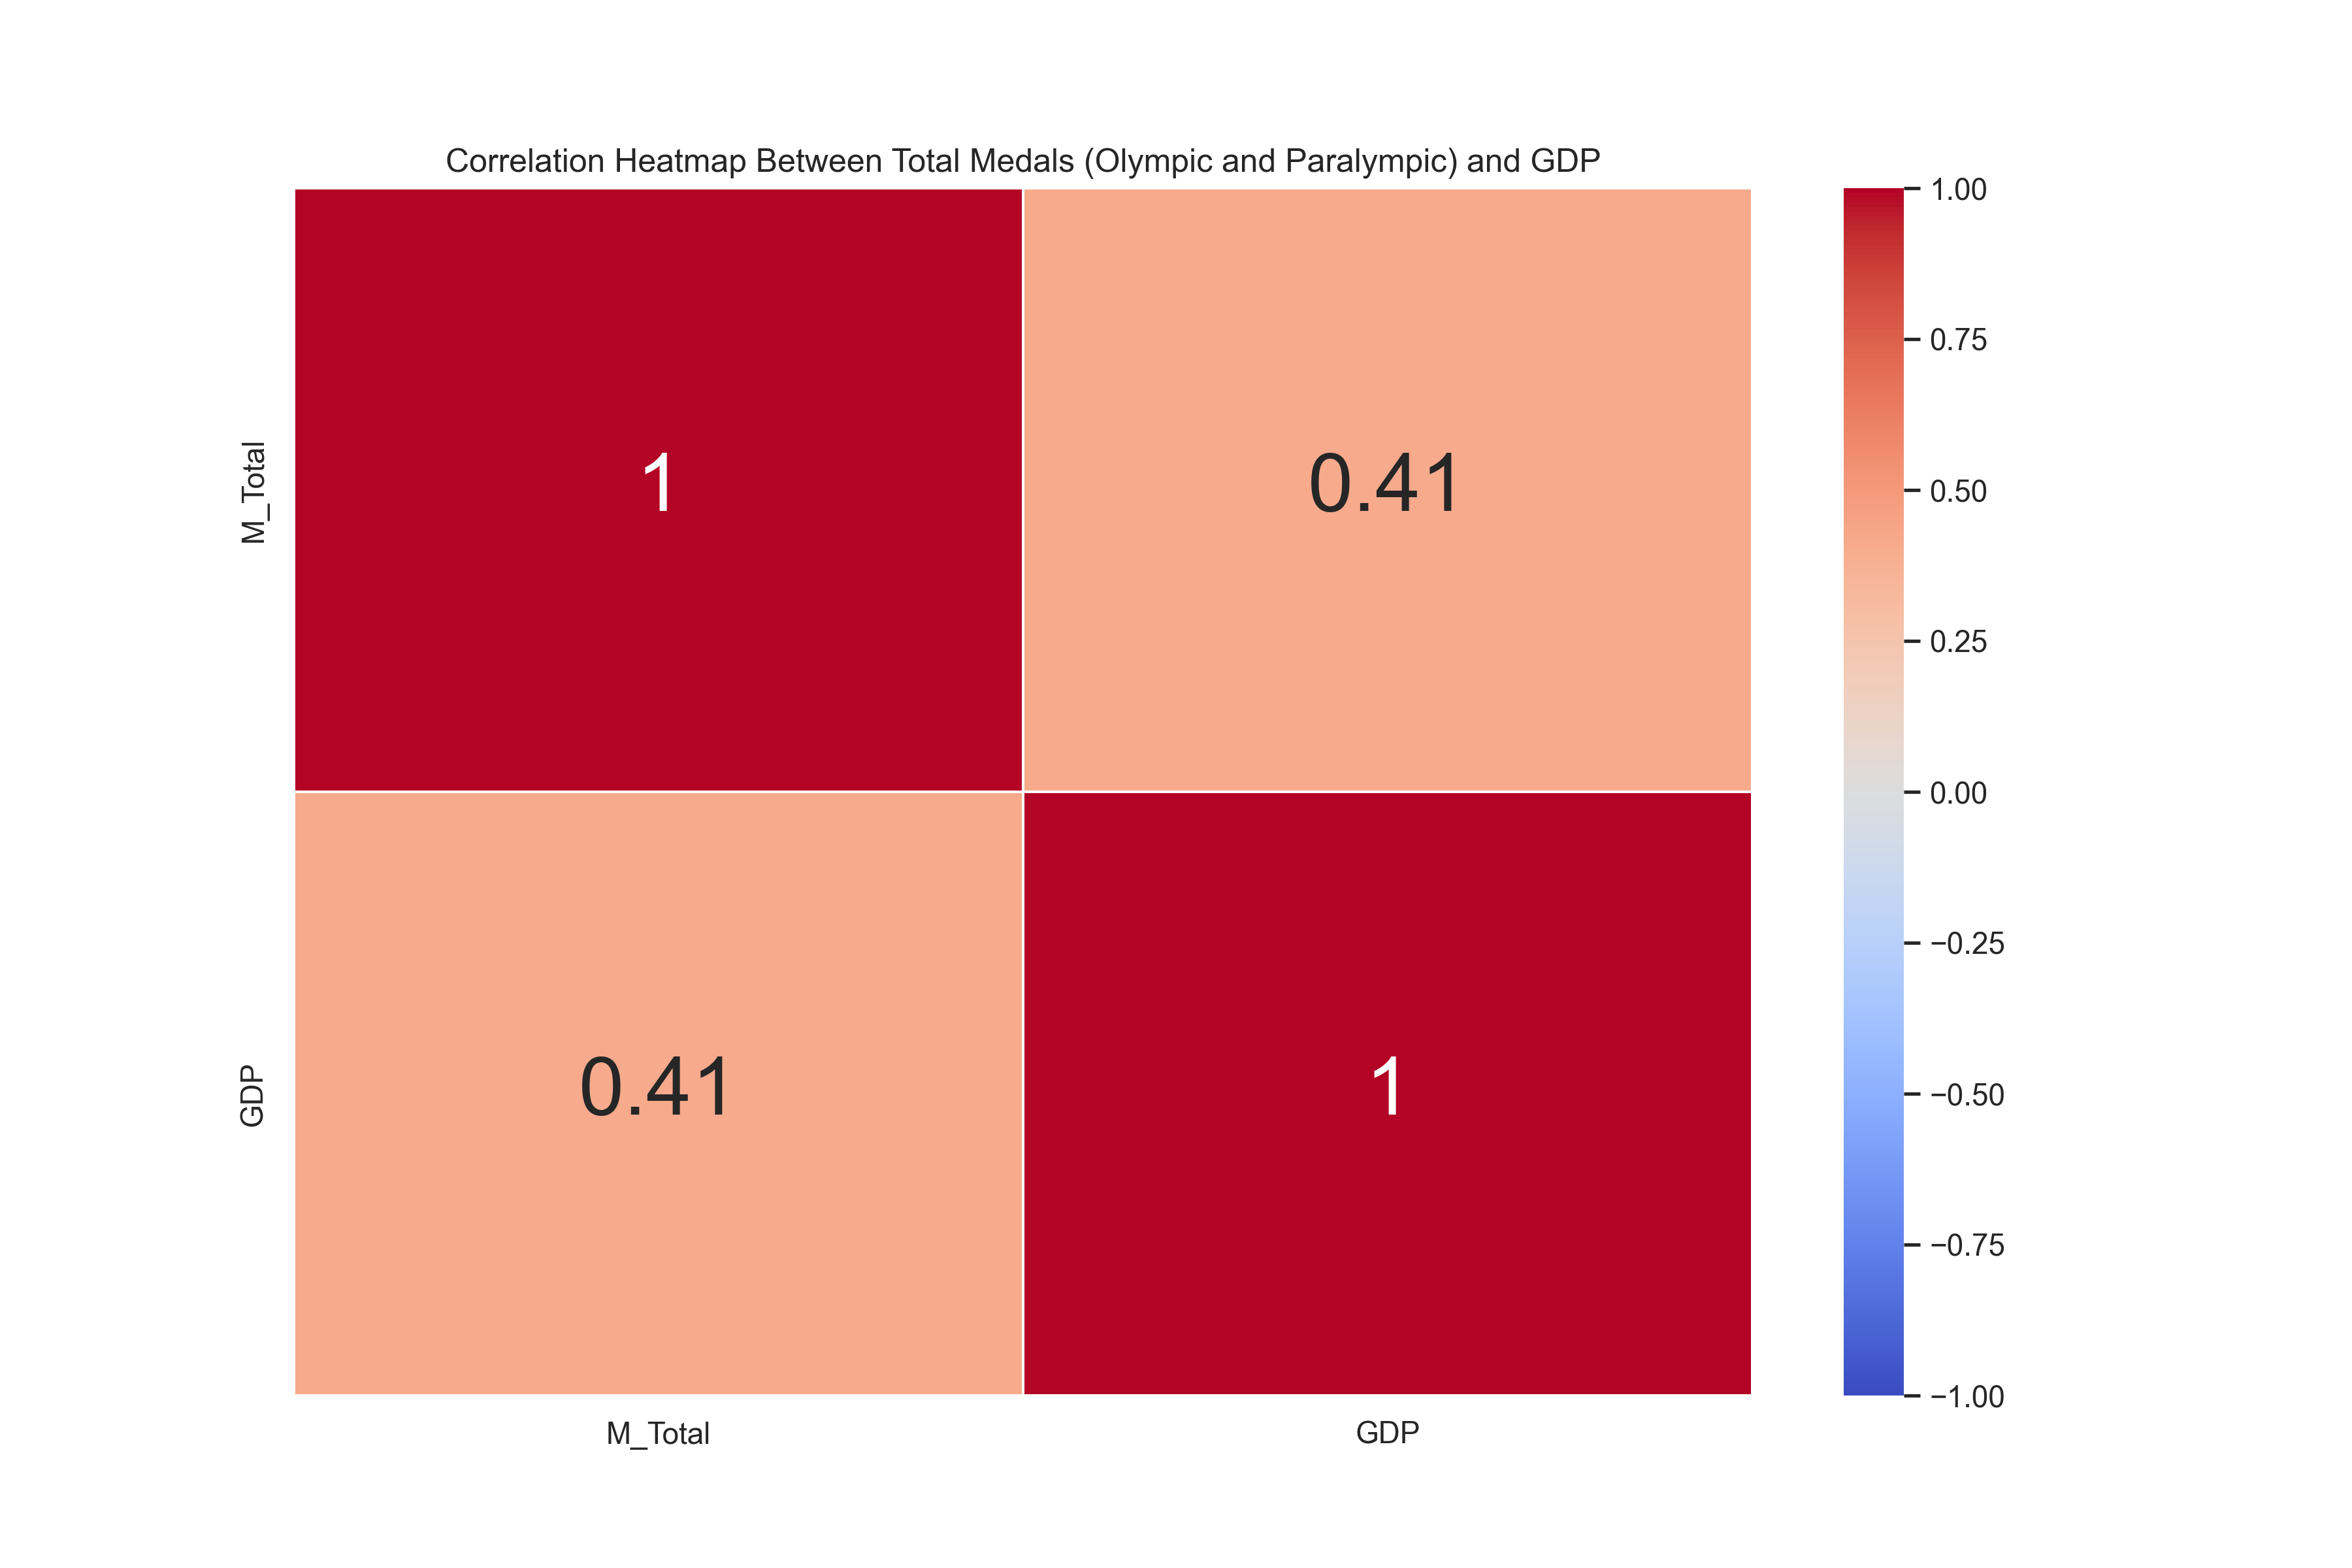
\includegraphics[width=\linewidth]{images/gdp_analysis/heatmap_total_medals_gdp.png}
        \caption{Correlation between Total Medals and GDP}
        \label{fig:medal_gdp_corr}
    \end{subfigure}
    \caption{Comparing Olympic and Paralympic Performance and GDP Influence}
    \label{fig:sidebyside_corr}
\end{figure}

Upon further examination of the relationship between GDP and the different types of medals (gold, silver, and bronze), subtle variations in correlation were identified, which point to the need for a more detailed analysis.

\begin{figure}[H]
    \centering
    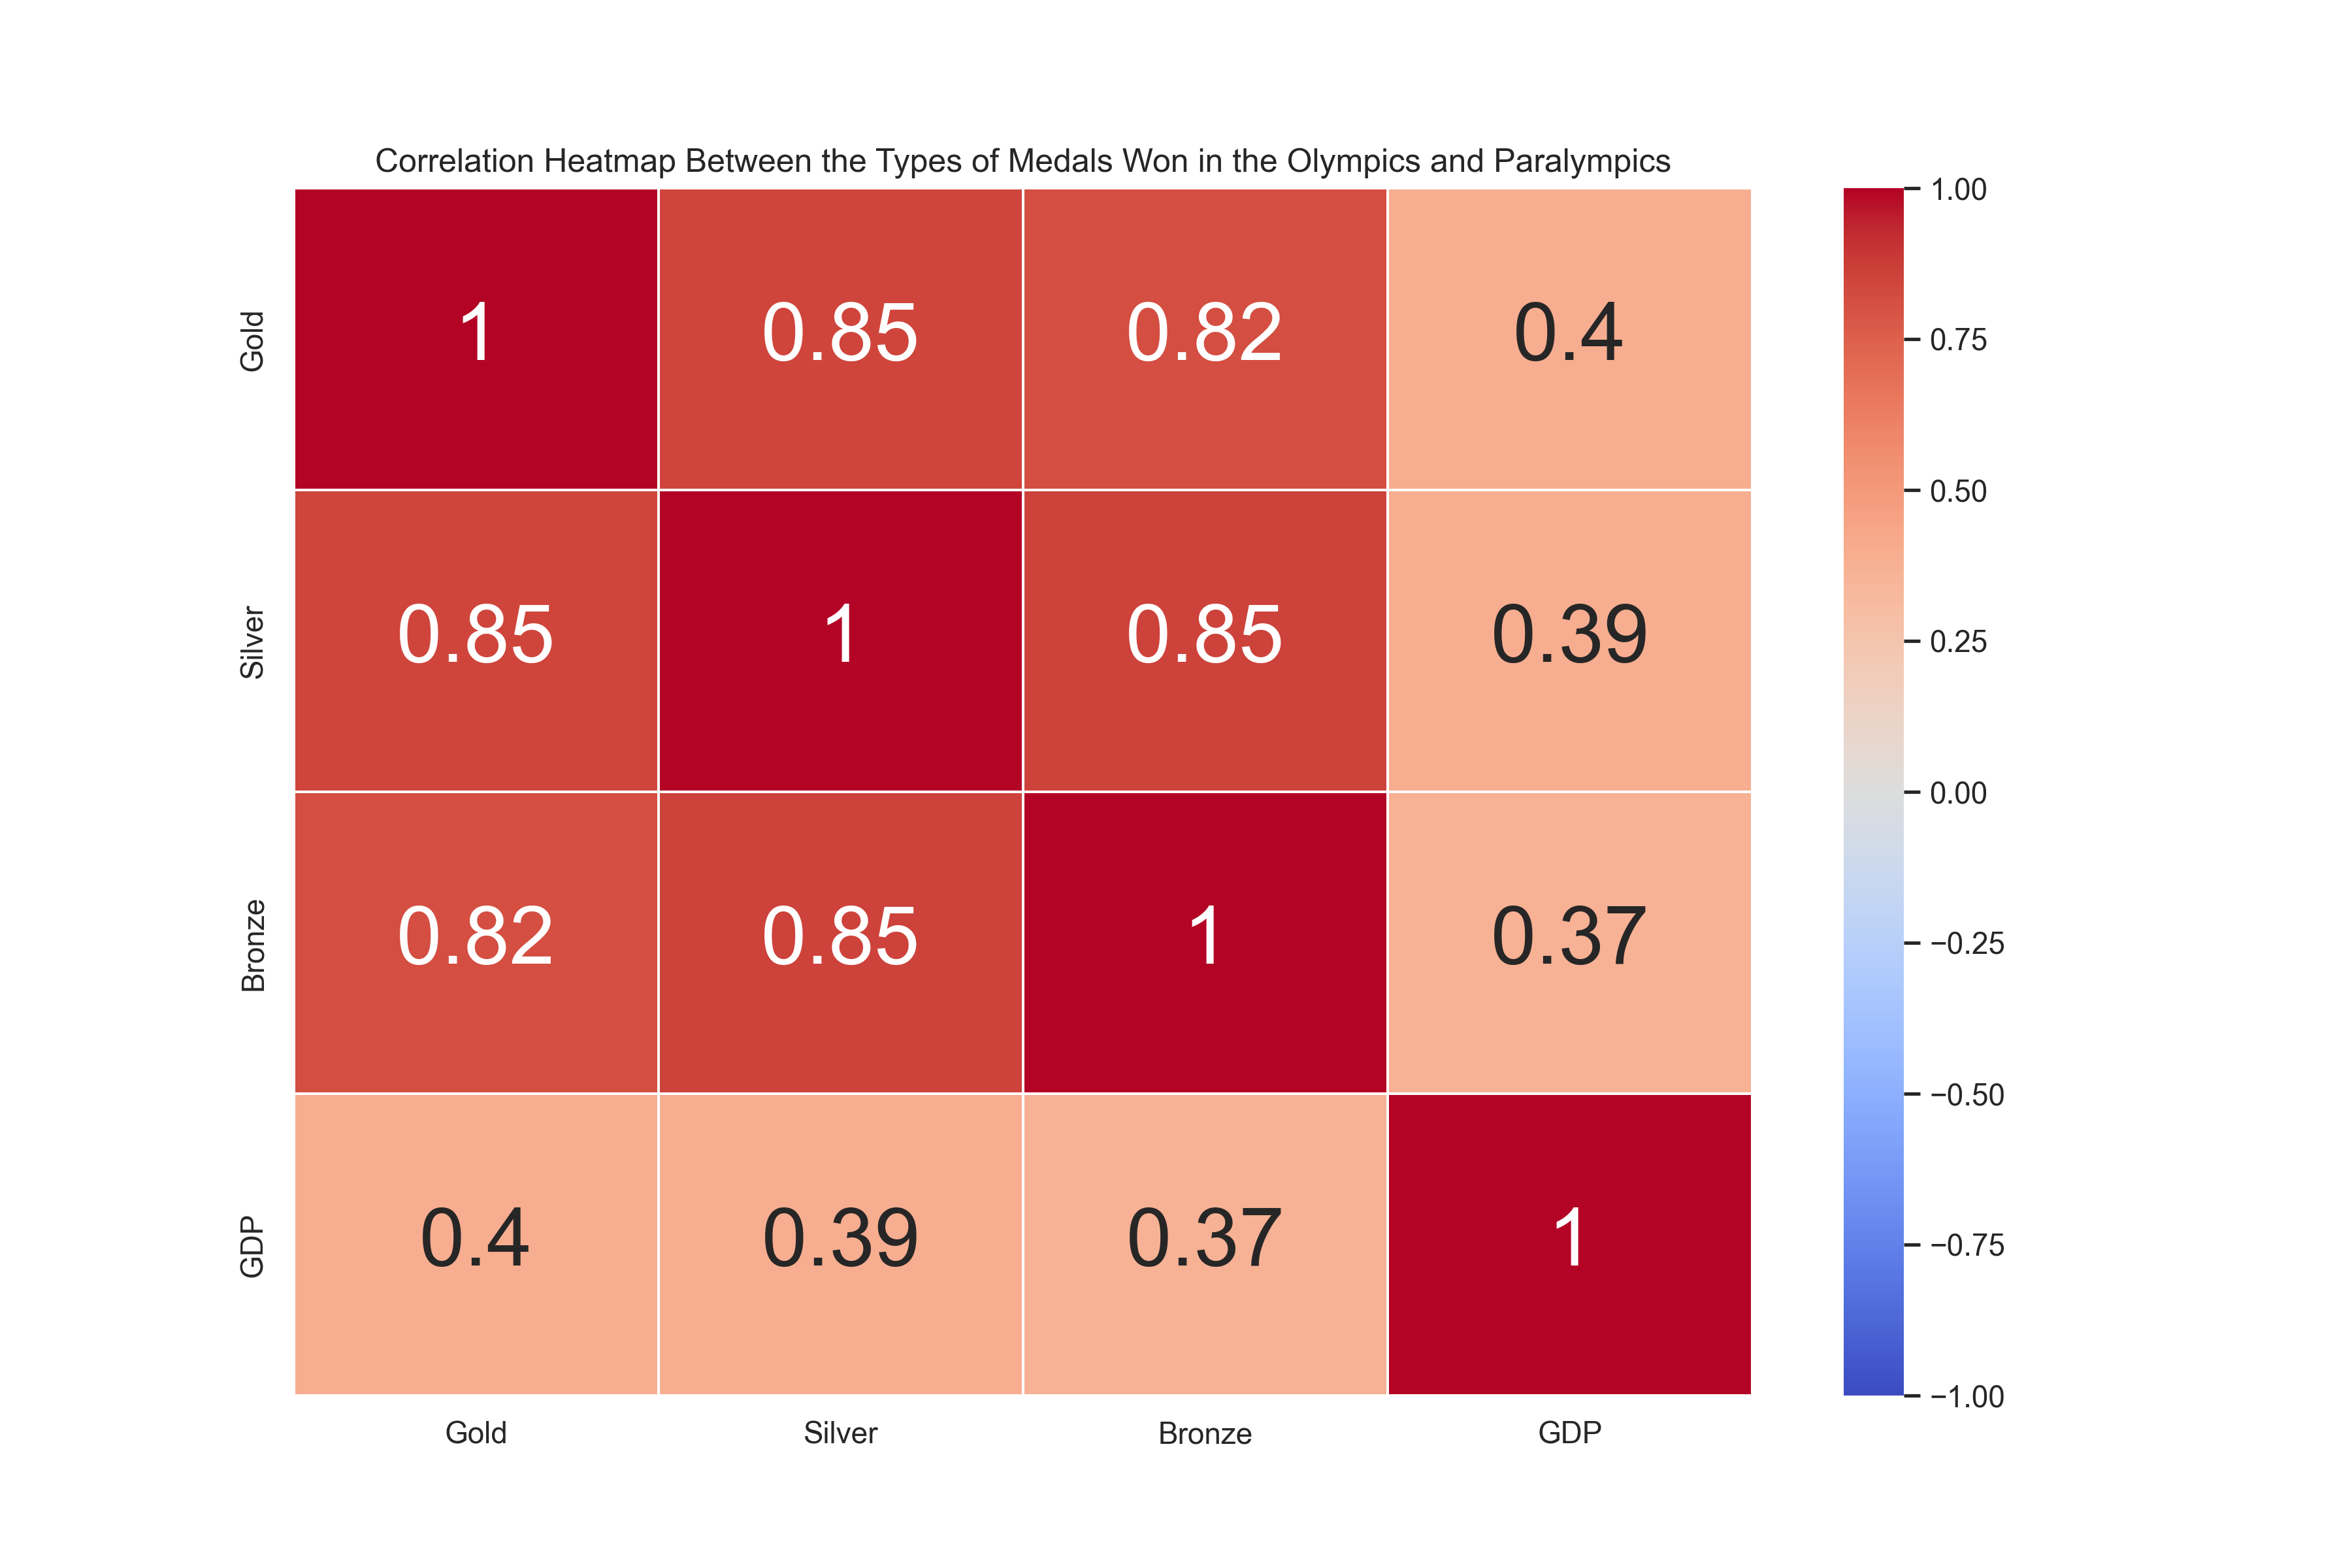
\includegraphics[width=0.6\linewidth]{images/gdp_analysis/heatmap_medals_categories_gdp.png}
    \caption{Correlation of Medal Types with GDP}
    \label{fig:medal_types_gdp_corr}
\end{figure}

To analyze the three variables simultaneously, the year 2016 was selected as it is the most recent year with complete data available. Below, a scatterplot is presented to show these relationships, followed by a zoomed-in version for better visualization.

\begin{figure}[H]
    \centering
    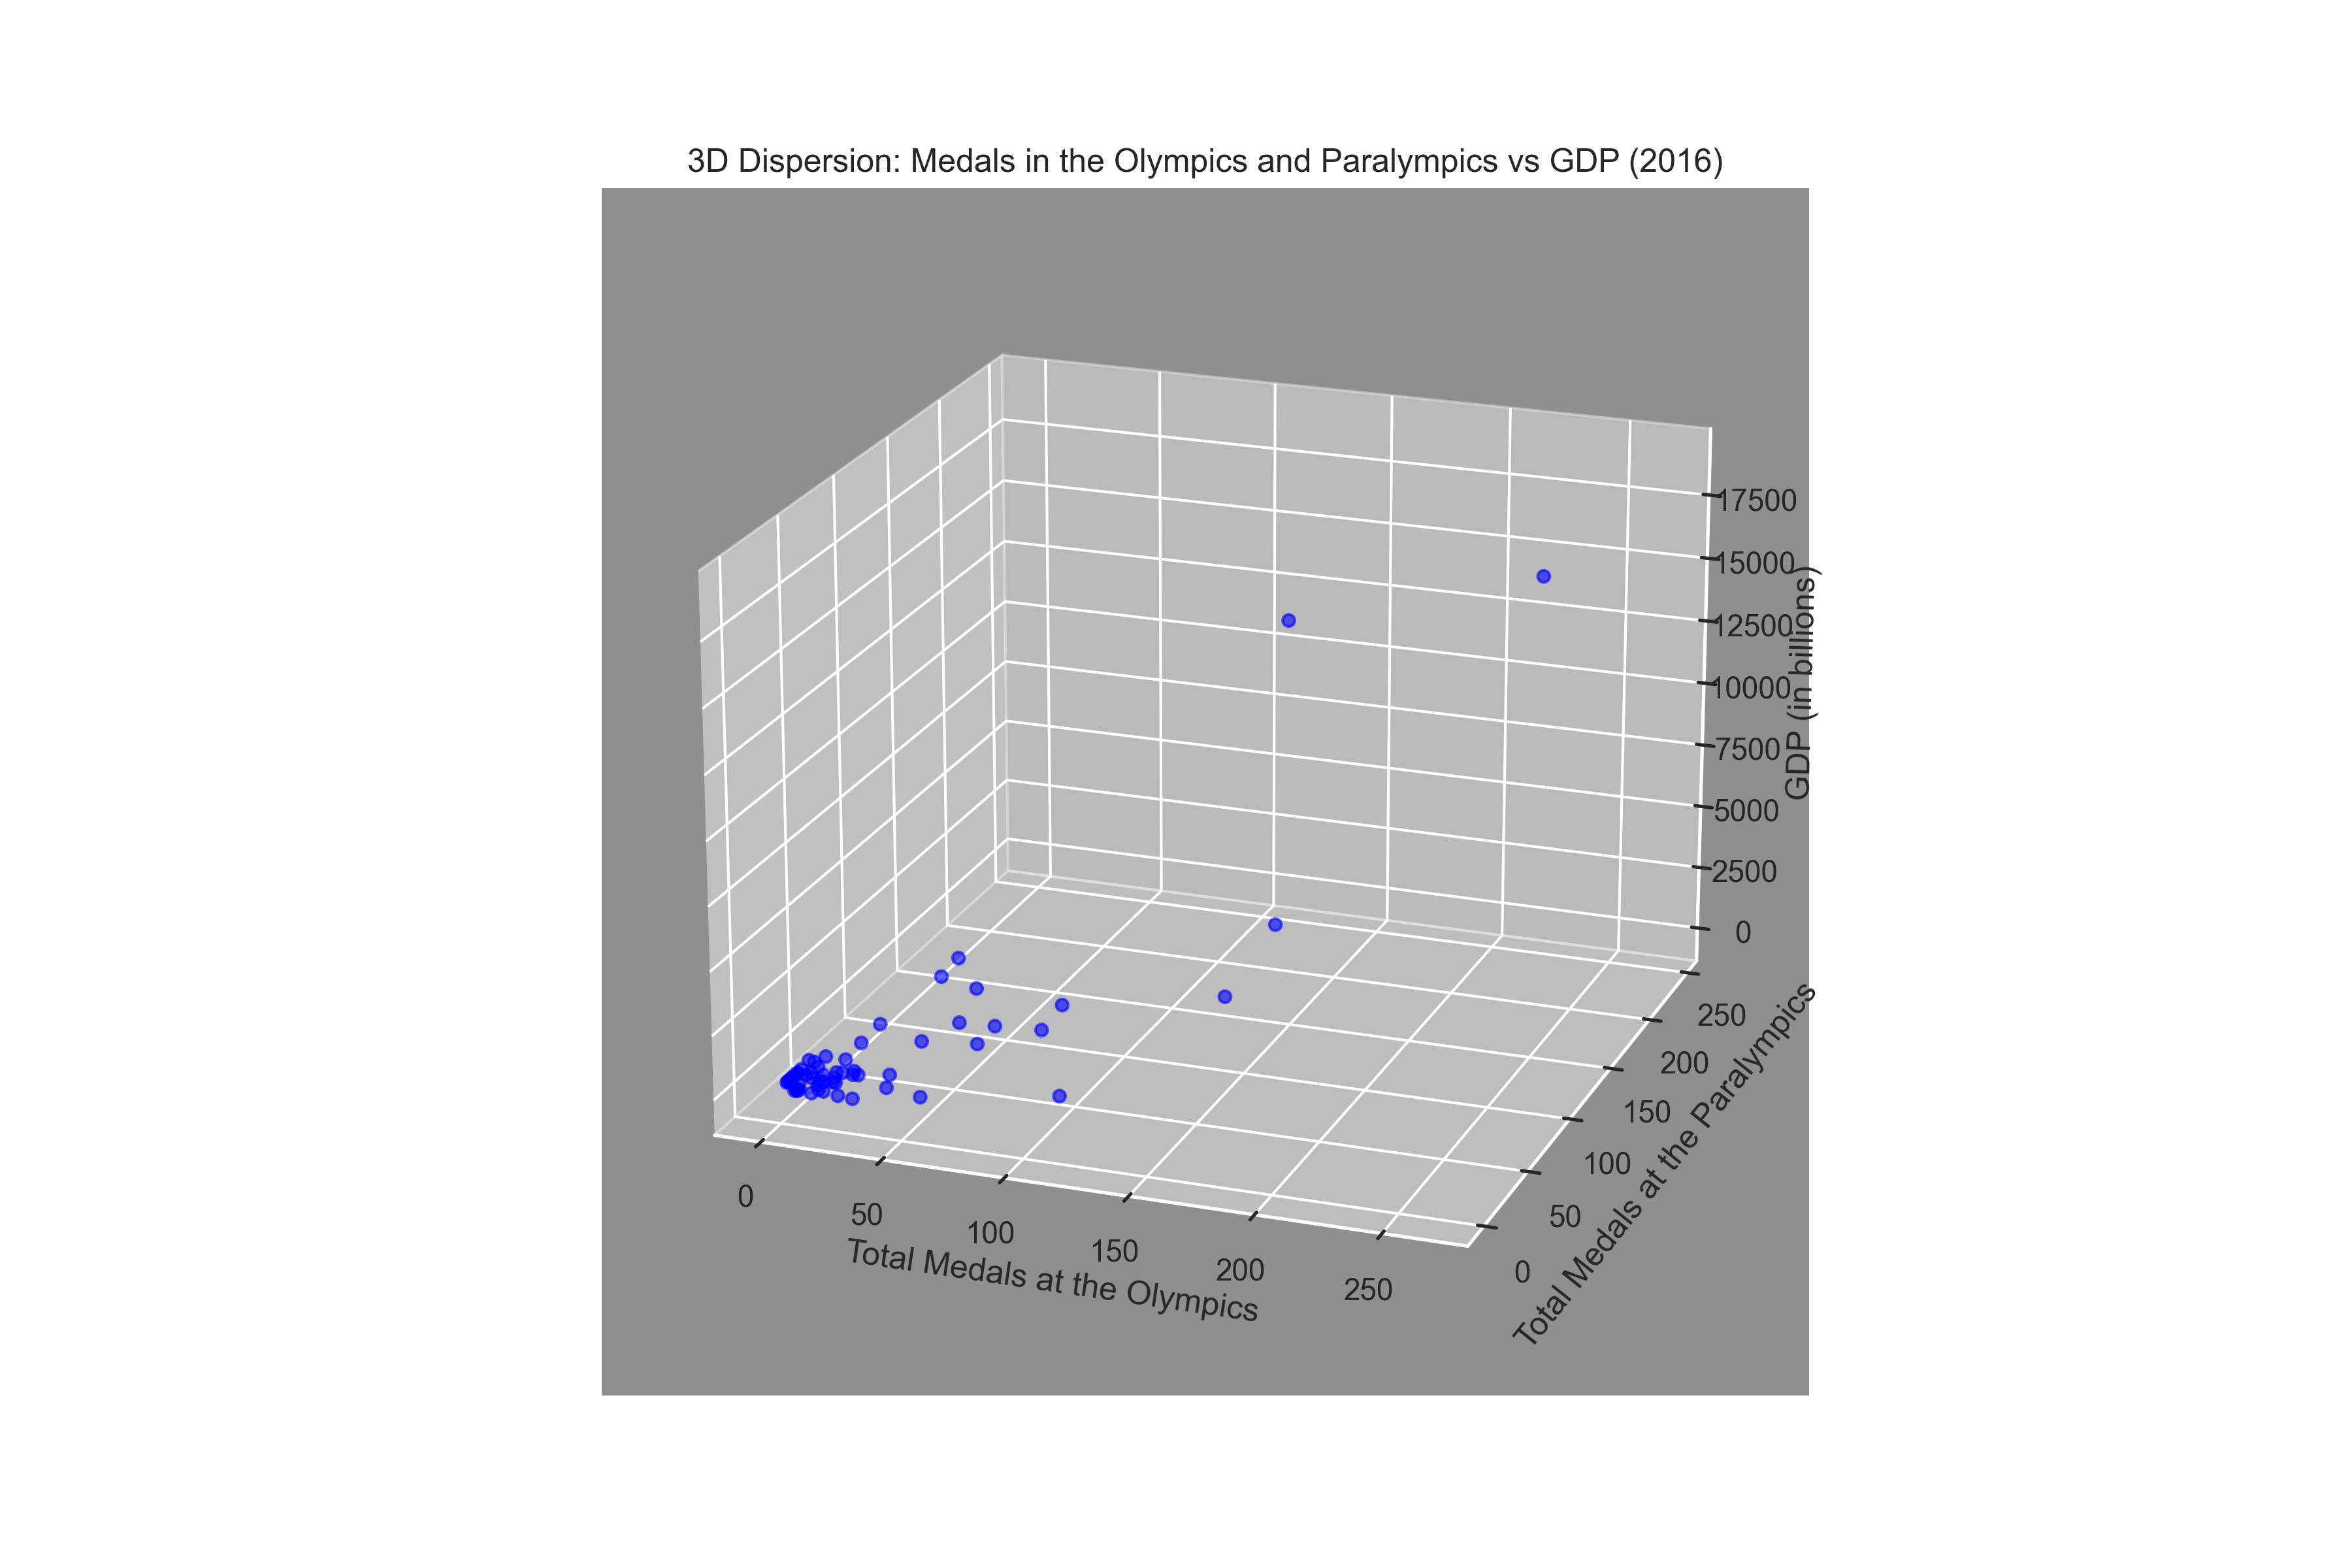
\includegraphics[width=\linewidth]{images/gdp_analysis/scatterplot_olympics_paralympics_pib_2016.png}
    \caption{Scatterplot for 2016: Olympic, Paralympic, and GDP}
    \label{fig:scatterplot_full}
\end{figure}

\begin{figure}[H]
    \centering
    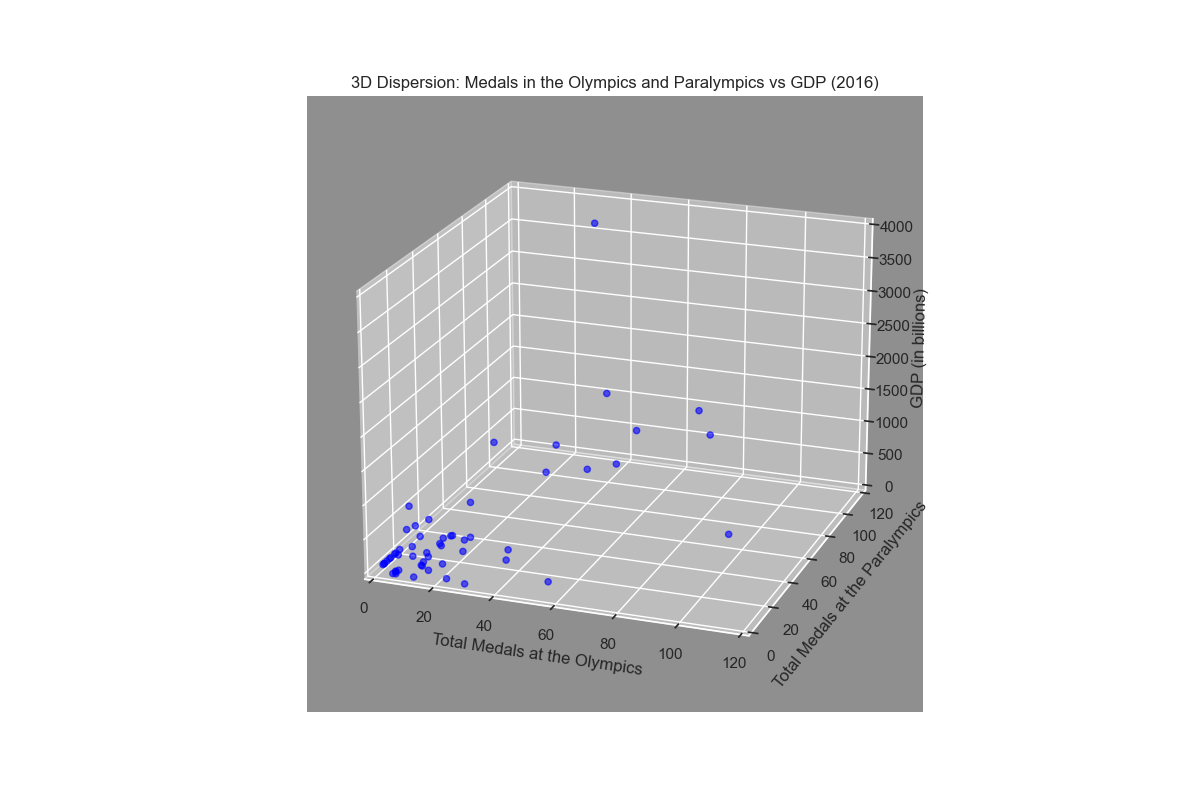
\includegraphics[width=\linewidth]{images/gdp_analysis/scatterplot_olympics_paralympics_pib_2016_approximate.png}
    \caption{Zoomed-In Scatterplot for 2016}
    \label{fig:scatterplot_zoomed}
\end{figure}

The analysis of these graphs reveals that while there is a strong relationship between Olympic and Paralympic performance, there is no significant correlation between these results and the GDP of the countries. This suggests that factors such as sports policies, athlete development programs, and targeted investments in specific sports are more critical determinants of medal success than economic strength alone.


\section{Conclusion and Future Work}
\subsection{Conclusion}

The analysis of Olympic and Paralympic data over the past 120 years has provided valuable insights into various dimensions of athlete performance, gender disparities, and the impact of external factors like urbanization and socioeconomic development.
\begin{itemize}
    \item Athlete Demographics and Performance: \begin{itemize}
        \item We found limited correlations between physical characteristics (age, height, and weight) and medal performance, particularly among Brazilian athletes, highlighting that while certain physical traits may provide advantages in specific sports, their influence on overall performance is marginal, most likely due to how there is a high amount of different competitions that may require different forms of training. \item There are hints that suggest that physical attributes are more closely related with the athletes' choice of sport rather than their competition results.
    \end{itemize}
    \item Gender Dynamics:
    \begin{itemize}
        \item The gender comparison revealed that, while the global performance of female athletes has steadily improved over time in both the Olympics and Paralympics, the trend in Brazil’s Paralympic data deviates from the global pattern, with noticeable fluctuations in performance. This points to the need for further investigation into the underlying causes of these variances, possibly linked to infrastructure, funding, or sociocultural factors affecting female participation in sports.
    \end{itemize}
    \item Impact of External Factors:
    \begin{itemize}
        \item Urbanization appeared to be loosely correlated with the success of countries in accumulating medals. Nations like China and Brazil, with rapid urban growth, showed corresponding increases in Olympic success. However, countries already highly urbanized (e.g., the U.S., Canada, and Germany) displayed different trajectories, suggesting that the relationship between urbanization and Olympic performance is context-specific.
        \item The same can be said about the correlation between the GDP of said country and its athletic performance. While there seems to be some sort of correlation, somewhat influenced by the amount of funds dedicated to sporting, it is irresponsible to presume causation of high athletic performance due to singularly the country's GDP.
    \end{itemize}
\end{itemize}

\subsection{Future Work}

\begin{itemize}
    \item Deepening the Gender Analysis
    \begin{itemize}
        \item While the initial gender comparison highlighted some key trends, future work could include a more granular analysis of individual sports, exploring whether certain sports have historically offered greater opportunities for female athletes, and whether differences in funding, training, or societal support influence gender-based performance trends.
    \end{itemize}
    \item Examining the Paralympic Variability
    \begin{itemize}
        \item The fluctuations in Paralympic performance, especially in Brazil, suggest that further work could focus on exploring specific factors driving these trends. It may be valuable to analyze policy changes, societal attitudes towards disabled athletes, and the allocation of resources to Paralympic programs in different regions.
    \end{itemize}
    \item Longitudinal Studies on Urbanization and Performance
    \begin{itemize}
        \item A more in-depth longitudinal study focusing on the relationship between urbanization and athletic performance could help clarify if urban growth directly influences sporting success, or if other mediating factors, like investment in sports infrastructure, play a larger role. Incorporating data on government spending and infrastructure development could enhance this analysis.
    \end{itemize}
    \item Exploring the Socioeconomic Divide in Sports Participation
    \begin{itemize}
        \item The analysis hinted at potential disparities in performance linked to economic conditions. Future work could investigate the role of income inequality, government funding for sports, and access to training facilities, particularly in less urbanized or developing nations.
    \end{itemize}
    \item Impact of Winter vs. Summer Games Participation
    \begin{itemize}
        \item There is a noticeable difference in the number of athletes participating in Winter versus Summer Games, which might affect the trends in medal accumulation and gender dynamics. Further analysis of how climate, regional focus on sports, and access to winter sports facilities impact participation and success would provide a more rounded understanding.
    \end{itemize}
\end{itemize}

\bibliographystyle{johd}
\bibliography{bib}


\end{document}